\chapter{Implementation}\label{cha:implementation}

A number of components were created to implement the proposed architecture. This chapter will provide a high level overview of the system, then examine each component in further detail.

\section{Overall Solution}
\begin{figure}[h]
	\centering
	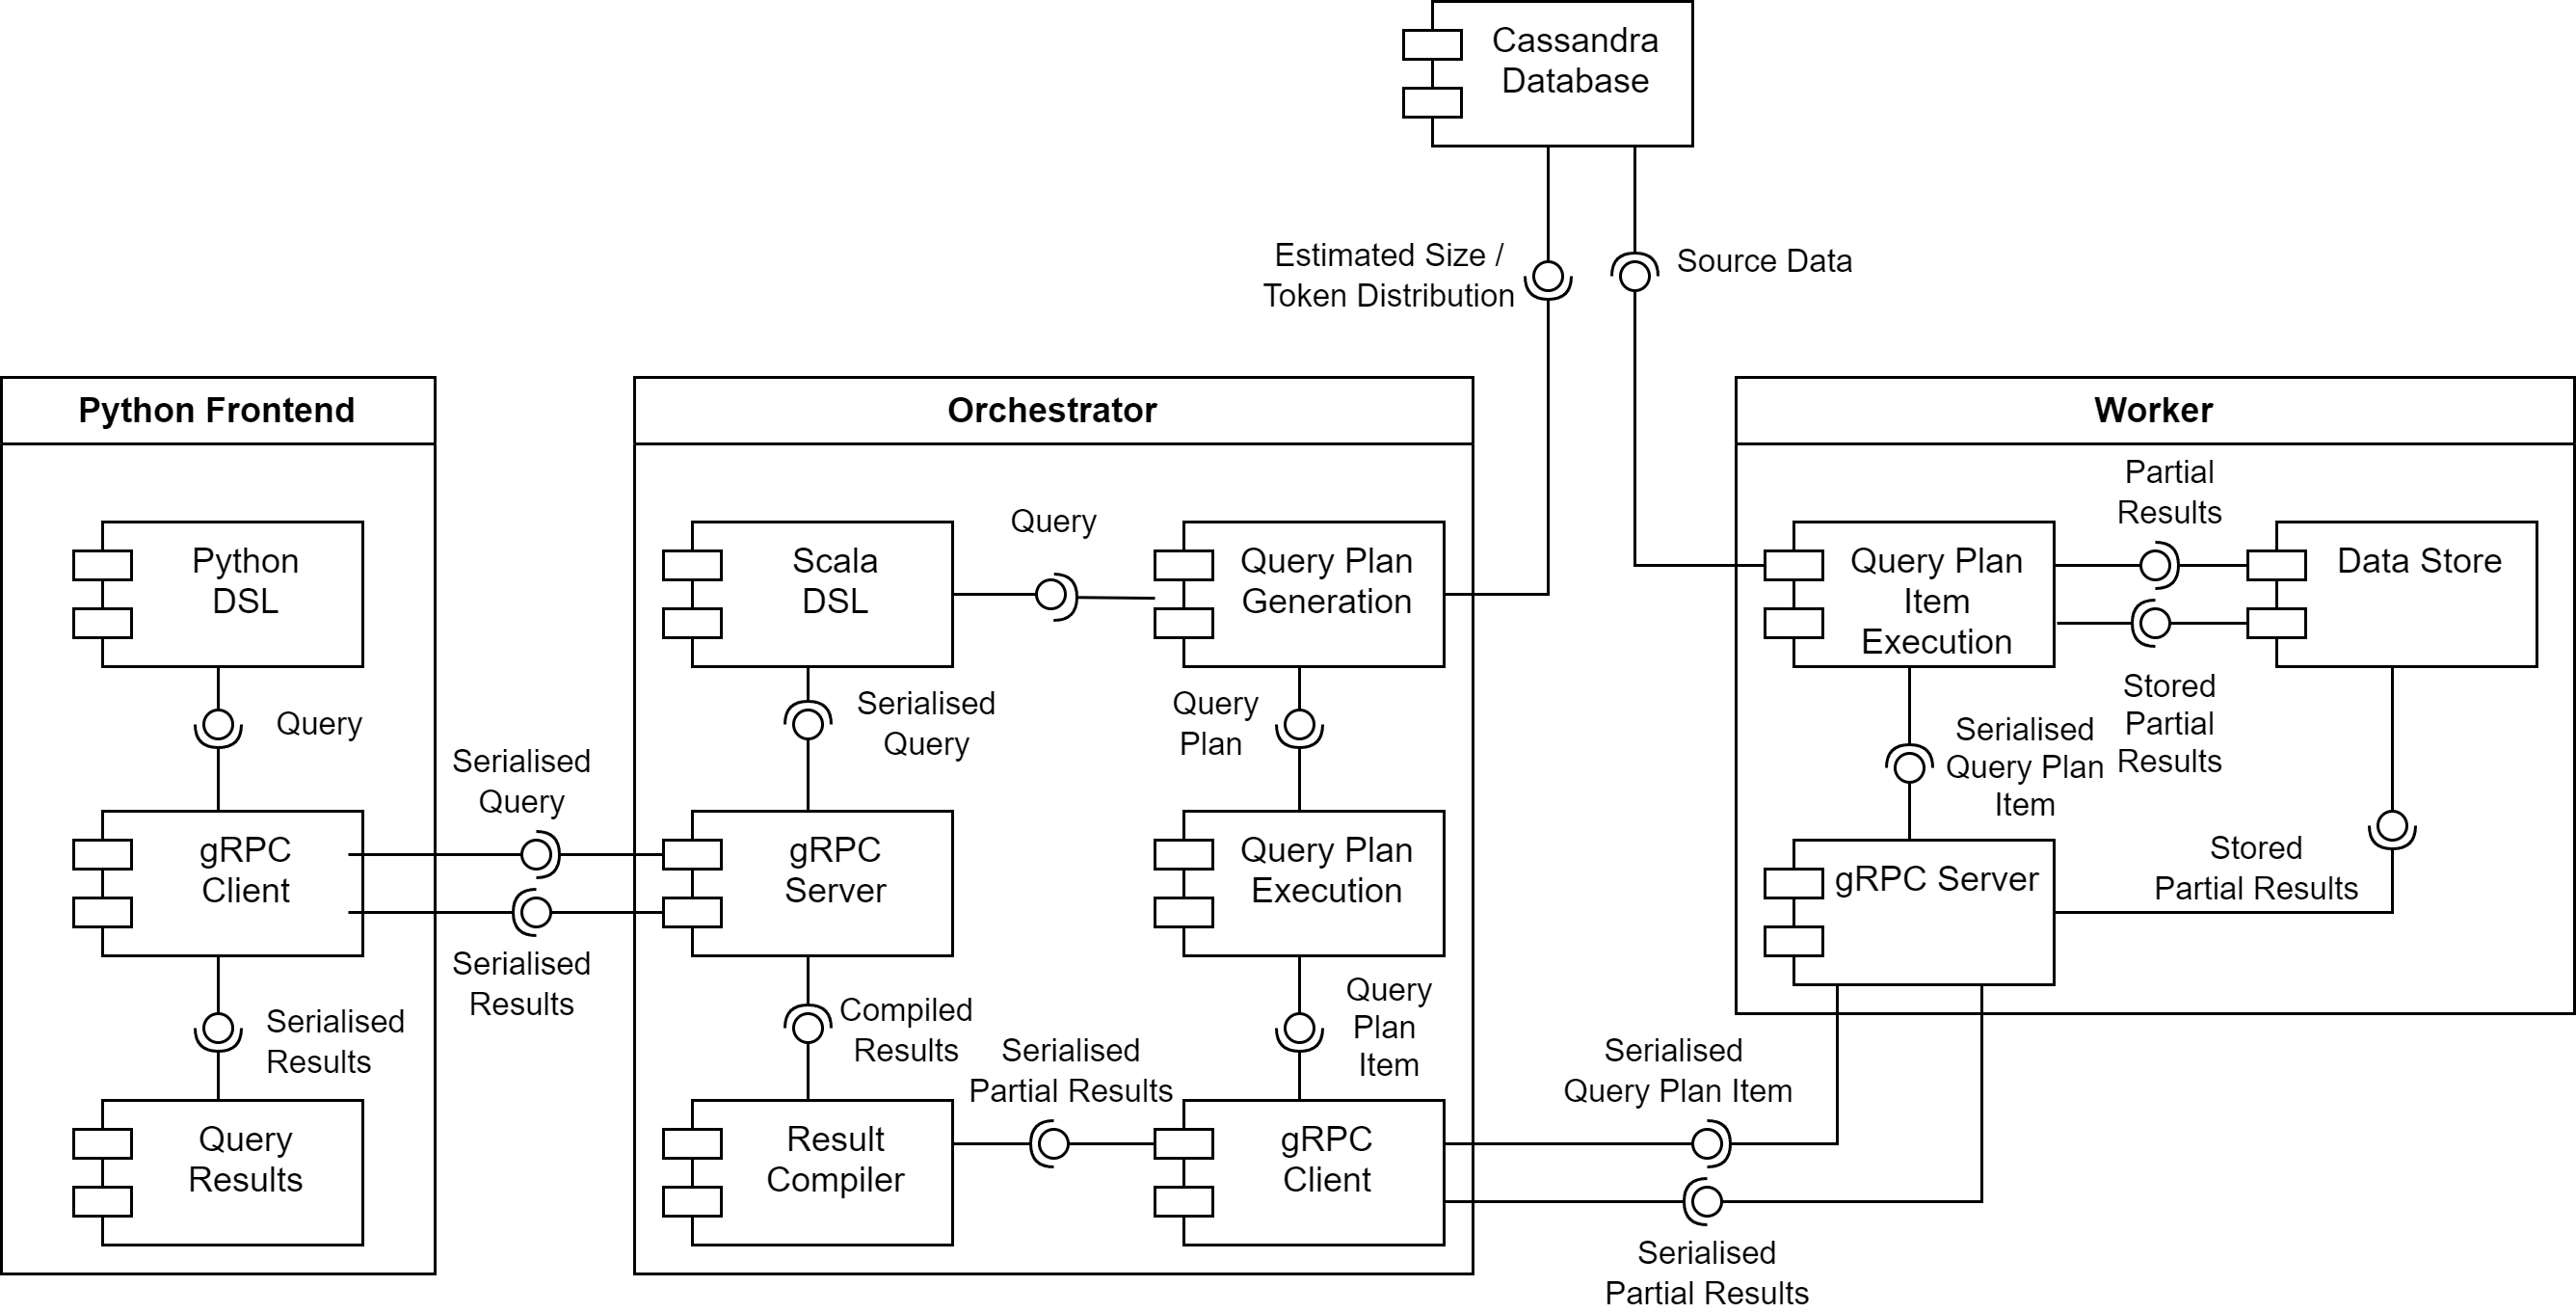
\includegraphics[width=0.7\textwidth]{chapters/diagrams/implementation/component-architecture-diagram}
	\caption{Solution Component Diagram}
	\label{fig:component-architecture-diagram}
\end{figure}

Figure \ref{fig:component-architecture-diagram} shows a component diagram for the core components, and their interactions. As described in Section \ref{sec:architecture}, the frontend is the user's entrypoint to the system. It acts as a terminal, allowing the user to define queries using the Python Domain Specific Language (DSL), and receive results. Queries are sent to the orchestrator, which acts as the central state management for the system. A number of components are used to get from query to result. First, it generates a query plan which describes the steps for computing a result. Then, the query plan is executed step-by-step, with the data used in each step being split up into a number of chunks of work (partitions) before being delegated to the workers. The workers are responsible for accepting these partitions, and performing the computation. Finally, when all query plan steps have been executed, the orchestrator fetches partial results from all workers, collates them into a final result, and returns this to the frontend. gRPC is used anywhere where network communication is required between the frontend, orchestrator and worker nodes.

The system supports three types of queries: Select, Filter and Group By. Both Select and Filter are row-level operations, meaning the workers do not have to pass data to one another during computation. However, Group By does need the workers to cross-communicate, which means they also require a temporary store to cache partial results.

\section{Type System}\label{sec:type-system}
The type system's role is to provide a representation for every type of value the user can store within a table. However, designing the interfaces to represent these values presents a challenge. Figure \ref{fig:type-system-motivation} demonstrates the problem. 

On the left, an example is shown where the table is a 2D list of raw values. As multiple types are stored in the same list, there is no shared type information between the values, so types cannot be used to determine the table's contents. To discover a value's type, the system would have to perform runtime type checks against all supported types, adding a significant amount of overhead. 

On the right, a conceptual model is shown, using a container class. The container holds a raw value with the type information about the value, and the table is a 2D list of containers. The system only needs to perform one runtime type check in order to instantiate the correct class instance. 

\begin{figure}[htp]
	\centering
	% left - data stored in raw format - no information 
	% right - data stored in containers with value and type information, can infer what type the value is from the stored type information
	\centering
	\subfloat[\centering Raw Data - No Type Information Available]{
		\begin{tabular}{r c c l}
			\textbf{Header:} [& id, & name & ] \\
			\textbf{Row 1:} [& 1, & "Alice" & ] \\
			\textbf{Row 2:} [& 2, & "Bob" & ] \\
		\end{tabular}
	}
	\qquad
	\subfloat[\centering Container Class - Value and Type Information Stored Together]{
		\begin{tabular}{r c c l}
			\textbf{Header:} [& (id, int), & (name, string) & ] \\
			\textbf{Row 1:} [& (1, int), & ("Alice", string) & ] \\
			\textbf{Row 2:} [& (2, int), & ("Bob", string) & ] \\
		\end{tabular}
	}
	\caption{Type System - Motivating Example}
	\label{fig:type-system-motivation}
\end{figure}

Due to Java limitations, this conceptual solution is not entirely straightforward to implement. The container class could use a generic type parameter which stores the type information of the value in the container, but generic type information is erased at runtime \cite{ghosh2004generics}. Instead, it could be defined as an interface, with each supported type providing an implementation of that interface, but this is not much better than the raw data solution, as the runtime type check simply becomes a pattern match on the class instance. A solution that exploits some kind of polymorphism is preferred. 

Scala provides a feature known as \textit{ClassTags} \cite{scalaclasstags}. These save the erased type information and also permit equality checks between \textit{ClassTag} instances, meaning the framework can use them to compare the type of a value to an expected type. The container class is therefore defined as an interface \textit{ValueType}, which holds a \textit{ClassTag} instance. This interface is implemented by \textit{TableField}, which holds field name and type, and \textit{TableValue}, which holds a value and its type. Concrete implementations for the 5 supported types, described in Section \ref{subsec:supported-types}, are provided for both subclasses. Figure \ref{fig:type-system-hierarchy} shows the class hierarchy.

\begin{figure}[htp]
	\centering
	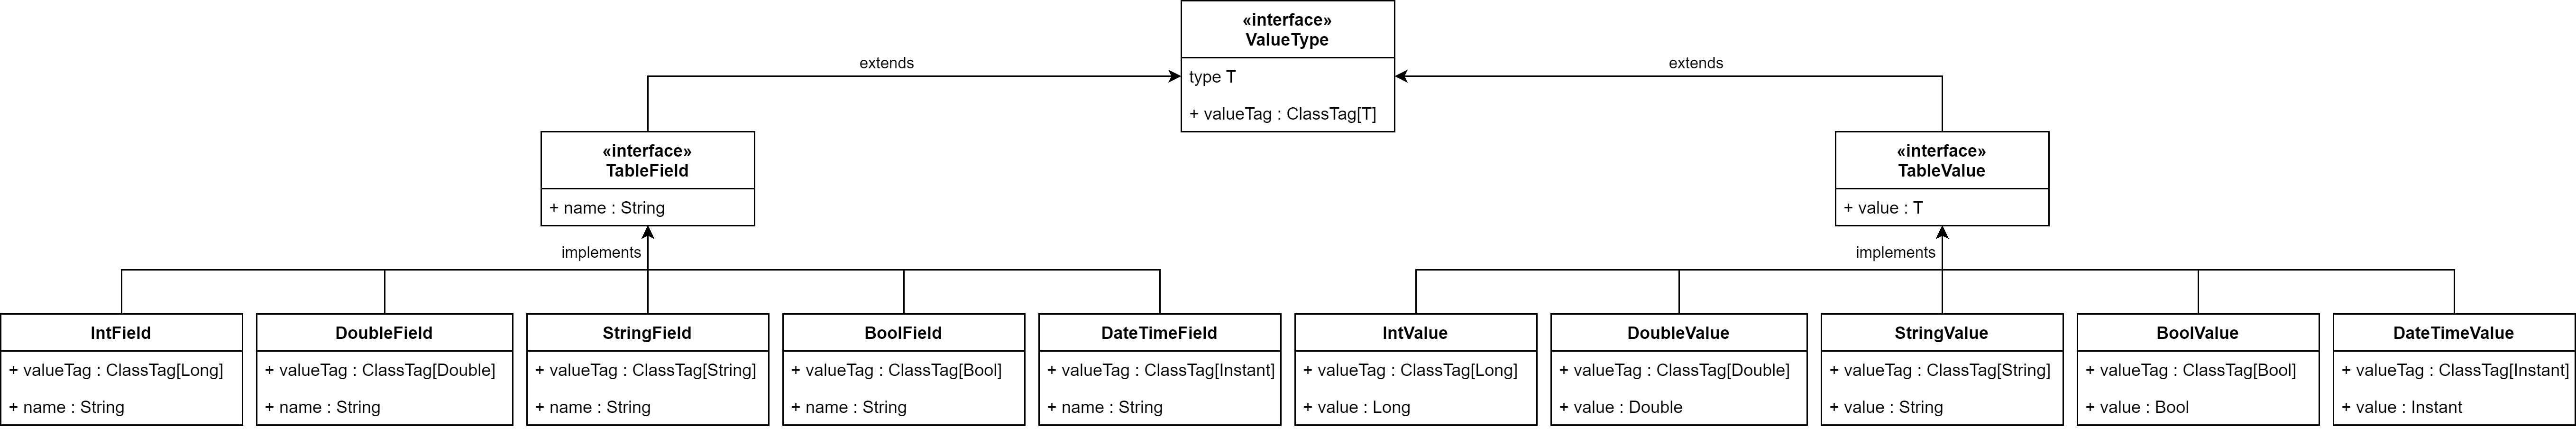
\includegraphics[width=0.7\textwidth]{chapters/diagrams/implementation/type-system-hierarchy}
	\caption{Custom Type System Hierarchy}
	\label{fig:type-system-hierarchy}
\end{figure}

\subsection{Supported Types}\label{subsec:supported-types}
The type system supports a subset of Scala, Python, and Cassandra's types, shown in Figure \ref{fig:datatypes}.

\begin{figure}[htp]
	\centering
	\begin{tabular}{| c | c | c | c |}
		\hline
		\textbf{Base Type} & \textbf{Python} & \textbf{Scala} & \textbf{Cassandra} \\ \hline
		Integer & int & Long & bigint \\ \hline
		Float & float & Double & double \\ \hline
		String & string & String & text \\ \hline
		Boolean & boolean & Boolean & boolean \\ \hline
		DateTime & datetime & Instant & timestamp \\ \hline
	\end{tabular}
	\caption{Primitive Types}
	\label{fig:datatypes}
\end{figure}

There were two main goals when selecting these primitive types. Firstly, every type should be able to be represented without data loss in all parts of the system. Secondly, it should be possible to represent the types in protobuf format, as this would allow for easy serialisation of result data. All types except DateTime can be converted to protobuf natively, and DateTimes are supported by serialising as an ISO8601 formatted string \cite{iso_8601}.

\subsection{Result Model}
The hierarchy of classes and supported types provide everything needed to define the result of a computation, known as a \textit{TableResult}. Headers are defined as a sequence of \textit{TableFields} and result rows are stored as a two-dimensional array of \texttt{Option[TableValue]}. As defined in the requirements, null values must be supported, but the use of nulls in Scala is discouraged. Instead, Option is preferred as it is supported by all the typical functional methods. In this model, values are represented by \texttt{Some(TableValue())}, and null values are represented by \texttt{Nothing}. Figure \ref{fig:example-table-result} shows what an example result looks like using this definition.

\begin{figure}[h]
	\centering
	\begin{tabular}{l c  c  c l}
		\textbf{Header:} [ & IntField(\textcolor{deepgreen}{"ID"}),  & StringField(\textcolor{deepgreen}{"Name"}),  & BoolField(\textcolor{deepgreen}{"Passed"}) & ] \\
		\textbf{Row 1:} [[ & Some(IntValue(1)), & Some(StringValue(\textcolor{deepgreen}{"Alice"})), & Some(BoolValue(true)) & ], \\
		\textbf{Row 2:}  [ & Some(IntValue(2)), & None, & None & ], \\
		\textbf{Row 3:}  [ & Some(IntValue(3)), & Some(StringValue(\textcolor{deepgreen}{"Bob"})), & None & ]] \\
	\end{tabular}
	\caption{Example Table Result}
	\label{fig:example-table-result}
\end{figure}

\section{Domain Specific Language}
The user's interaction with the framework is driven entirely by the Domain Specific Language (DSL), which is modelled with SQL-like syntax. The language allows users to define expressions, then use these in computations like Select, Filter and Group By. Figure \ref{fig:dsl-high-level-example} provides a sample annotated DSL query, with links to the sections where each part is discussed.

\begin{figure}[htp]
	Initialise cluster connection and select a Cassandra source table:
	\begin{python}
ClusterManager("orchestrator-url")
  .cassandra_table("example", "table")
	\end{python}
	
	Select query, uses \textit{FieldExpressions} (Section \ref{subsec:fieldexpressions}) and Python Operators (Section \ref{subsec:dsl-python}):
	\begin{python}
  .select(
    F("id"),
    (F("duration") * 2).as_name("duration2"),
    Function.Left(Function.ToString(F("date")), 8)
      .as_name("yyyy-mm")
  )
	\end{python}

	Filter query, uses \textit{FieldComparisons} (Section \ref{subsec:fieldcomparisons}) and Python Operators (Section \ref{subsec:dsl-python}):
	\begin{python}
  .filter(
    (F("duration2") > 40) && 
  	(F("yyyy-mm").contains("2021")
  )
	\end{python}

	Group By query, uses \textit{AggregateExpressions} (Section \ref{subsec:aggregateexpressions}):
	\begin{python}
  .group_by(
    [F("duration2")],
    [
      Max(F("id")),
      Count(F("yyyy-mm"))
    ]
  )
	\end{python}
	\caption{Example DSL Query}
	\label{fig:dsl-high-level-example}
\end{figure}


\subsection{FieldExpressions}\label{subsec:fieldexpressions}
\textit{FieldExpressions} are a key part of the DSL, allowing the user to define arbitrary row-level calculations to be used as part of more complex operations. They are defined as an interface, with three subclasses:

\begin{itemize}
	\item Values: define literal values which never change across all rows
	\item Fields: get the value from the given field name in the current row.
	\item FunctionCalls: perform arbitrary function calls using further FieldExpressions as arguments.
\end{itemize}

Figure \ref{fig:field-expressions-examples} provides examples for each type of \textit{FieldExpression}.

\begin{figure}[htp]
	Values (from left to right): string "a", integer 1, double 1.5, boolean True, date 31/12/2021.
	\begin{python}
V("a") , V(1), V(1.5), V(True), V(datetime.date(2021, 12, 31))
	\end{python}

	Fields (from left to right): fieldName, duration, id, creationDate.
	\begin{python}
F("fieldName"), F("duration"), F("id"), F("creationDate")
	\end{python}

	Top Function: convert 'field1' to a string, then take the left 10 characters of each row.
	
	Bottom Function: multiply 'field2' by 2, then divide by "field3"
	\begin{python}
Function.Left(Function.ToString(F("field1")), 10)
(F("field2") * 2) / F("field3")
	\end{python}
	\caption{\textit{FieldExpression} implementations and examples}
	\label{fig:field-expressions-examples}
\end{figure}

Many basic functions have been implemented, including arithmetic, string and cast operations. ver, the function system is designed to be extensible. A number of helper classes are defined to allow the creation of basic unary, binary and ternary functions, but \textit{FunctionCall} is itself an interface which can be given completely custom implementations if required. The main constraint on the functions that can be defined are that only the 5 primitive input types are supported.

\paragraph{Type Resolution} 
Type Resolution on FieldExpressions is performed in two stages: a resolution step, and an evaluation step. The resolution step takes in type information from a \textit{ClassTag} in the header of the input result, and verifies that the \textit{FieldExpression} is well-typed with regards to that result; see Section \ref{sec:type-system} for details. The evaluation step performs the computation on a row from that result without any type checking. Unchecked casts are used here instead, demonstrated for a binary function in Figure \ref{fig:fieldexpression-unchecked-casts}. 

\begin{figure}[htp]
	\centering
	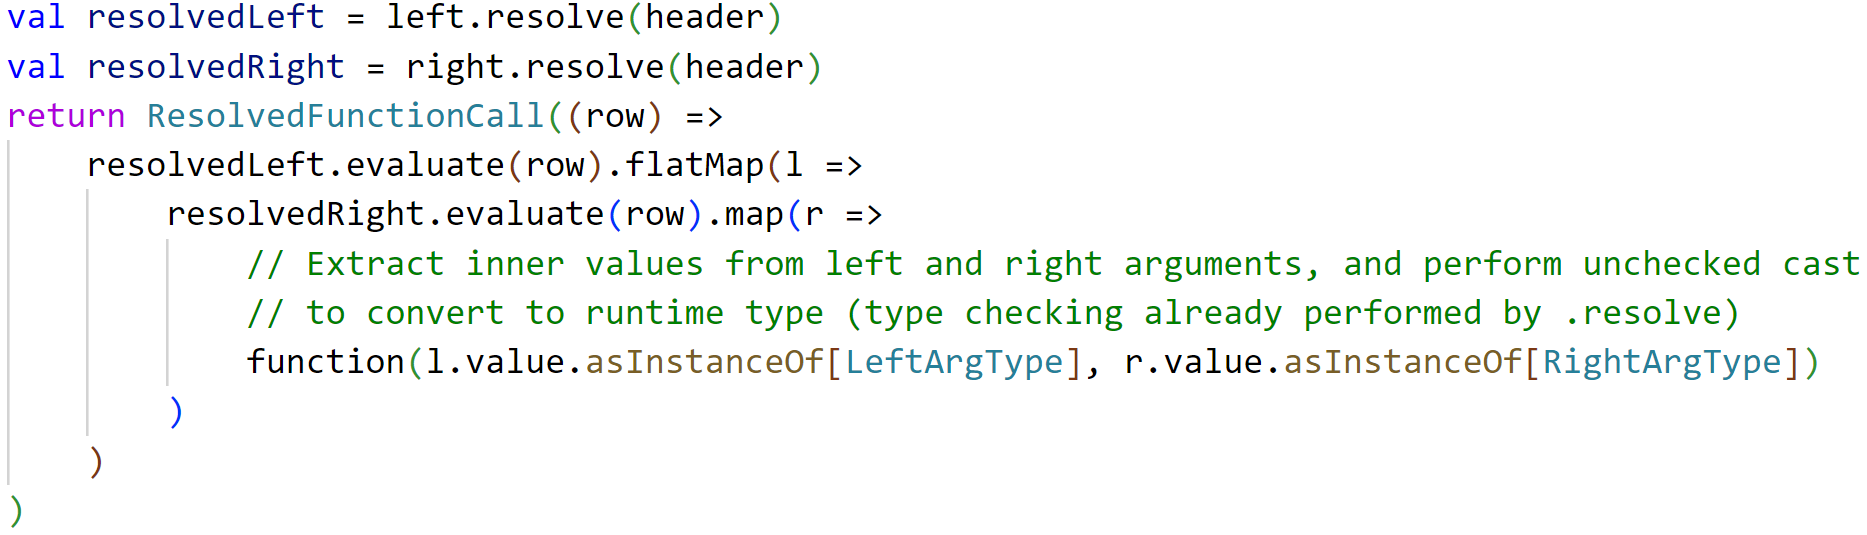
\includegraphics[width=\textwidth]{chapters/diagrams/implementation/type-resolution-unchecked-casts}
	\caption{Runtime Evaluation of Functions}
	\label{fig:fieldexpression-unchecked-casts}
\end{figure}

There are two main situations where the resolution step catches errors. Firstly, a Field reference is invalid if the field name is not present in the table header, shown in Figure \ref{fig:field-type-resolution}. Secondly, a Function call is invalid if an argument returns an invalid type, shown in Figure \ref{fig:function-type-resolution}.

\begin{figure}[htp]
	\centering
	For the expression F(\textcolor{deepgreen}{"field"}):
	
	\subfloat[\centering Valid - \textcolor{deepgreen}{"field"} is present in the header]{
		\begin{tabular}{l c l}
			\textbf{Header:} [& IntField(\textcolor{deepgreen}{"field"}) ] \\
		\end{tabular}
	}
	\qquad
	\subfloat[\centering Invalid - \textcolor{deepgreen}{"field"} not present in the header]{
		\begin{tabular}{l c l}
			\textbf{Header:} [& StringField(\textcolor{deepgreen}{"differentField"}) ] \\
		\end{tabular}
	}
	\caption{Type Resolution of Fields}
	\label{fig:field-type-resolution}
\end{figure}

\begin{figure}[htp]
	Valid - both arguments to \textit{Concat} are strings:
	\begin{python}
Function.Concat(V("hello"), V("Alice"))
	\end{python}
	
	Invalid - \textit{V(1)} is not a string:
	\begin{python}
Function.Concat(V("hello"), V(1))
	\end{python}
	\caption{Type Resolution of Functions}
	\label{fig:function-type-resolution}
\end{figure}


A two-step process has a number of benefits. The resolution step enables a form of polymorphism on some functions like arithmetic operations. These determine what types are returned by their sub-expressions during resolution, resolving to the correct version for evaluation. For example, the add function resolves to \textit{AddInt}, \textit{AddDouble}, or \textit{Concat}. It also reduces the overhead at runtime as type checking does not need to be performed for each row.

\paragraph{Named Expressions}
When performing a Select operation, the output fields are all expected to be named. This allows the user to chain operations by referencing fields from the previous input. Figure \ref{fig:namedfieldexpression-examples} shows the two ways of naming a field: \textit{FieldExpressions} can be assigned a user-defined name, or \textit{F()} expressions will also keep their name automatically.

\begin{figure}[htp]
	Top Expression Name: 'twice\textunderscore duration'
	
	Bottom Expression Name: 'creation\textunderscore date'
	\begin{python}
(F("duration") * 2).as_name("twice_duration")
F("creation_date")
	\end{python}
	\caption{\textit{NamedFieldExpression} examples}
	\label{fig:namedfieldexpression-examples}
\end{figure}

\subsection{FieldComparisons}\label{subsec:fieldcomparisons}
\textit{FieldComparisons} are another key building block of the DSL, allowing the user to define arbitrary row-level comparisons. \textit{FieldComparisons} use a two-step resolution-evaluation process to accommodate the same process as \textit{FieldExpressions}. They are defined as an interface, with a number of comparison types implemented already, including null, equality, numerical and string comparisons. Examples of each are shown in Figure \ref{fig:field-comparisons-examples}.

\begin{figure}[htp]
	Null checks: verify whether an expression is null or not null.
	\begin{python}
F("duration").is_null()
F("duration").is_not_null()
	\end{python}
	
	Equality checks: verify whether two \textit{FieldExpressions} are equal or not equal. 
	\begin{python}
F("duration") == 20
F("duration") != F("other_duration")
	\end{python}

	Ordering checks: apply ordered comparators between two \textit{FieldExpressions}.
	\begin{python}
F("duration") < 20
F("duration") <= 19
F("duration") > 20
F("duration") >= 21
	\end{python}

	String checks: apply contains, starts with and ends with operators (case insensitive versions also available).
	\begin{python}
F("name").contains("Alice")
F("name").starts_with("Bob")
F("name").ends_with("Smith")
	\end{python}
	\caption{\textit{FieldComparison} examples}
	\label{fig:field-comparisons-examples}
\end{figure}

\paragraph{Combined Comparisons}
The user is able to combine multiple FieldComparisons using AND/OR operators, shown in Figure \ref{fig:field-comparisons-combiners}. This is a lightweight wrapper around Scala's own AND (\texttt{\&\&}) and OR (\texttt{||}) boolean operators, meaning optimisations like short circuiting operate as normal.

\begin{figure}[htp]
	\begin{python}
(F("duration") < 20) && (F("name").starts_with("Bob"))
(F("duration") < 20) || (F("name").starts_with("Bob"))
(F("duration") < 20) && (
  (F("name").contains("Bob")) || (F("name").contains("Alice"))
)
	\end{python}
	\caption{\textit{FieldComparison} AND/OR Combinations}
	\label{fig:field-comparisons-combiners}
\end{figure}

\subsection{Aggregate Expressions}\label{subsec:aggregateexpressions}
\textit{AggregateExpressions} are the final part of the DSL. These are used only as part of Group Bys, and allow the user to define methods of aggregating all rows of a result. They take a \textit{NamedFieldExpression} as an argument, and compute a single row output from any number of input result rows.

The supported operations are Minimum, Maximum, Sum, Average, Count, and String Concatenation, and they are polymorphic where possible. For example, minimum and maximum handle numeric types by ordering numerically and string types lexicographically. Figure \ref{fig:aggregate-expressions-examples} shows examples of \textit{AggregateExpressions}.

\begin{figure}[htp]
	\begin{python}
Max(Function.ToString(F("date")).as_name("date_string"))
Max(F("duration"))
Sum(F("amount"))
Count(F("id"))
	\end{python}
	\caption{\textit{AggregateExpression} examples}
	\label{fig:aggregate-expressions-examples}
\end{figure}

\subsection{Protocol Buffer Serialisation}
All components of the DSL have been designed to be serialised to protobuf format. This allows any queries written by the user to be passed around the system using gRPC, and if required the query can also be serialised to a file. The results of a query are also serialisable, to allow the system to return query results to the user. gRPC has a size limit of 4MB for individual messages, so results are split up by row and streamed individually.

\subsection{Python Implementation}\label{subsec:dsl-python}
The Python frontend is designed to be straightforward to use, hiding the complexities of the computation being performed in the backend. A number of Python-specific features were used to help with this.

Python allows developers to override common operators, including arithmetic and comparison, with custom definitions. The Python implementation of \textit{FieldExpression} overrides the arithmetic operators, as well as comparison operators to allow the user to automatically generate functions and \textit{FieldComparisons}, without having to write the full definition.

Furthermore, as discussed in \ref{subsec:frontend-design}, pandas is widely used for data analysis in Python \cite{reback2020pandas}. The frontend is able to convert query results from their protobuf definition to a pandas DataFrame to allow further analysis to be performed immediately.



\section{Data Model}\label{subsec:data-model}
% This section should be clear and understandable, as much of the rest refers to partial and full versions
The data model is split into two key components: \textit{DataSource} and \textit{Table}. 

\textit{DataSource} is an interface, representing any part of the query where data must be rearranged into new partitions, including Cassandra source data, and Group By operations. \textit{Table} is a class, representing any part of the query containing purely row-level computations, including Select and Filter operations. It is composed of a \textit{DataSource} and a list of row-level computations known as \textit{TableTransformations}. To compute its output, the \textit{DataSource} is computed first, then all transformations are applied sequentially.

Optionally, \textit{DataSources} can have dependent \textit{Tables} which must be calculated first. For example, a Group By \textit{DataSource} requires a single \textit{Table} to be fully computed before it can be generated. A Cassandra \textit{DataSource} will always act as the terminal component for a query, as it has no dependencies.

For demonstration purposes, Figure \ref{fig:filter-select-query} shows a Filter and Select query in the DSL, and the data model. Note that any number of Select and Filter operations can be placed in the Table component, as no new partitions are required to produce the result.

\begin{figure}[htp]
	\centering
	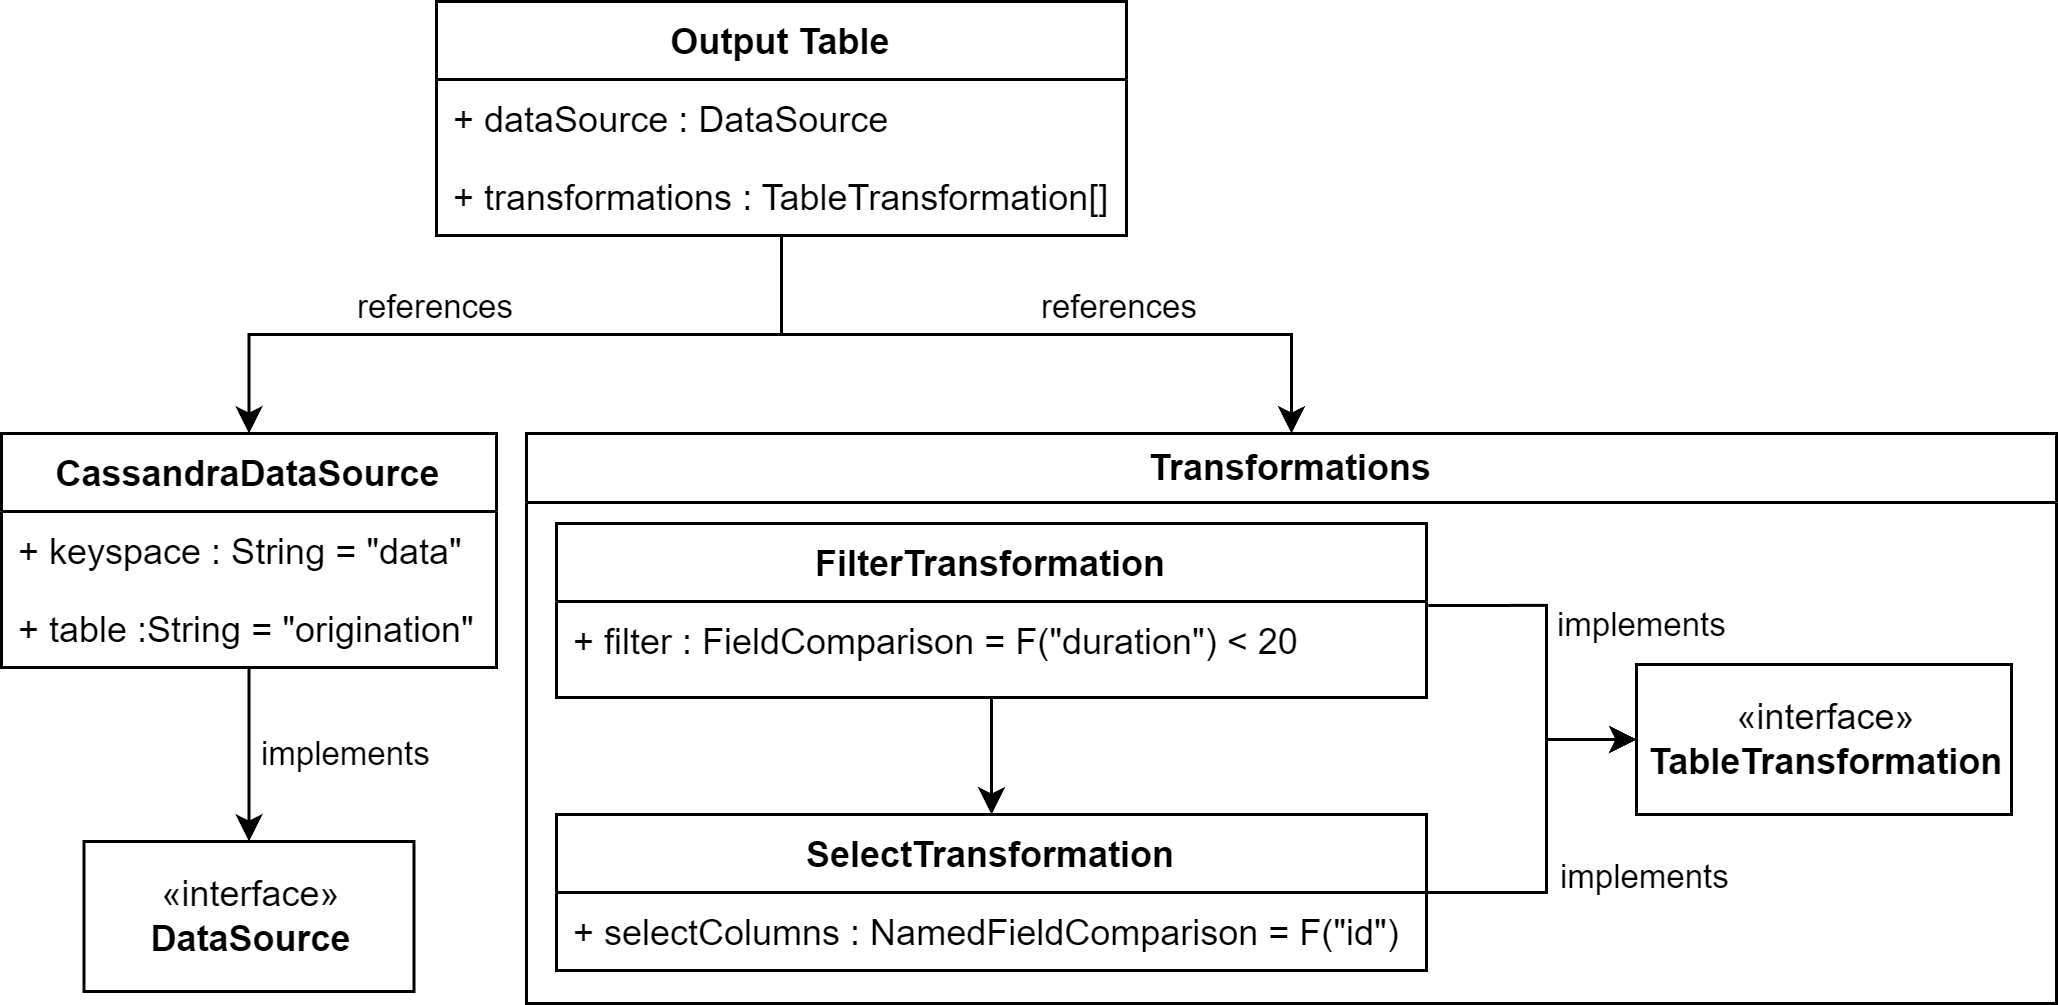
\includegraphics[width=0.8\textwidth]{chapters/diagrams/implementation/filter-select-query}
	\begin{python}
ClusterManager("orchestrator-service")
.cassandra_table("data", "origination")
.filter(F("duration") < 20)
.select(F("id"))
.evaluate()
	\end{python}
	\caption{Example Filter and Select Query}
	\label{fig:filter-select-query}
\end{figure}


Figure \ref{fig:group-by-query} shows a more complex query containing a Group By in the DSL, and the data model. The dependent table (bottom left) is calculated first, and its output is used to compute the Group By, in \textit{GroupByDataSource}. The final output is then generated in the output table.

\begin{figure}[htp]
	\centering
	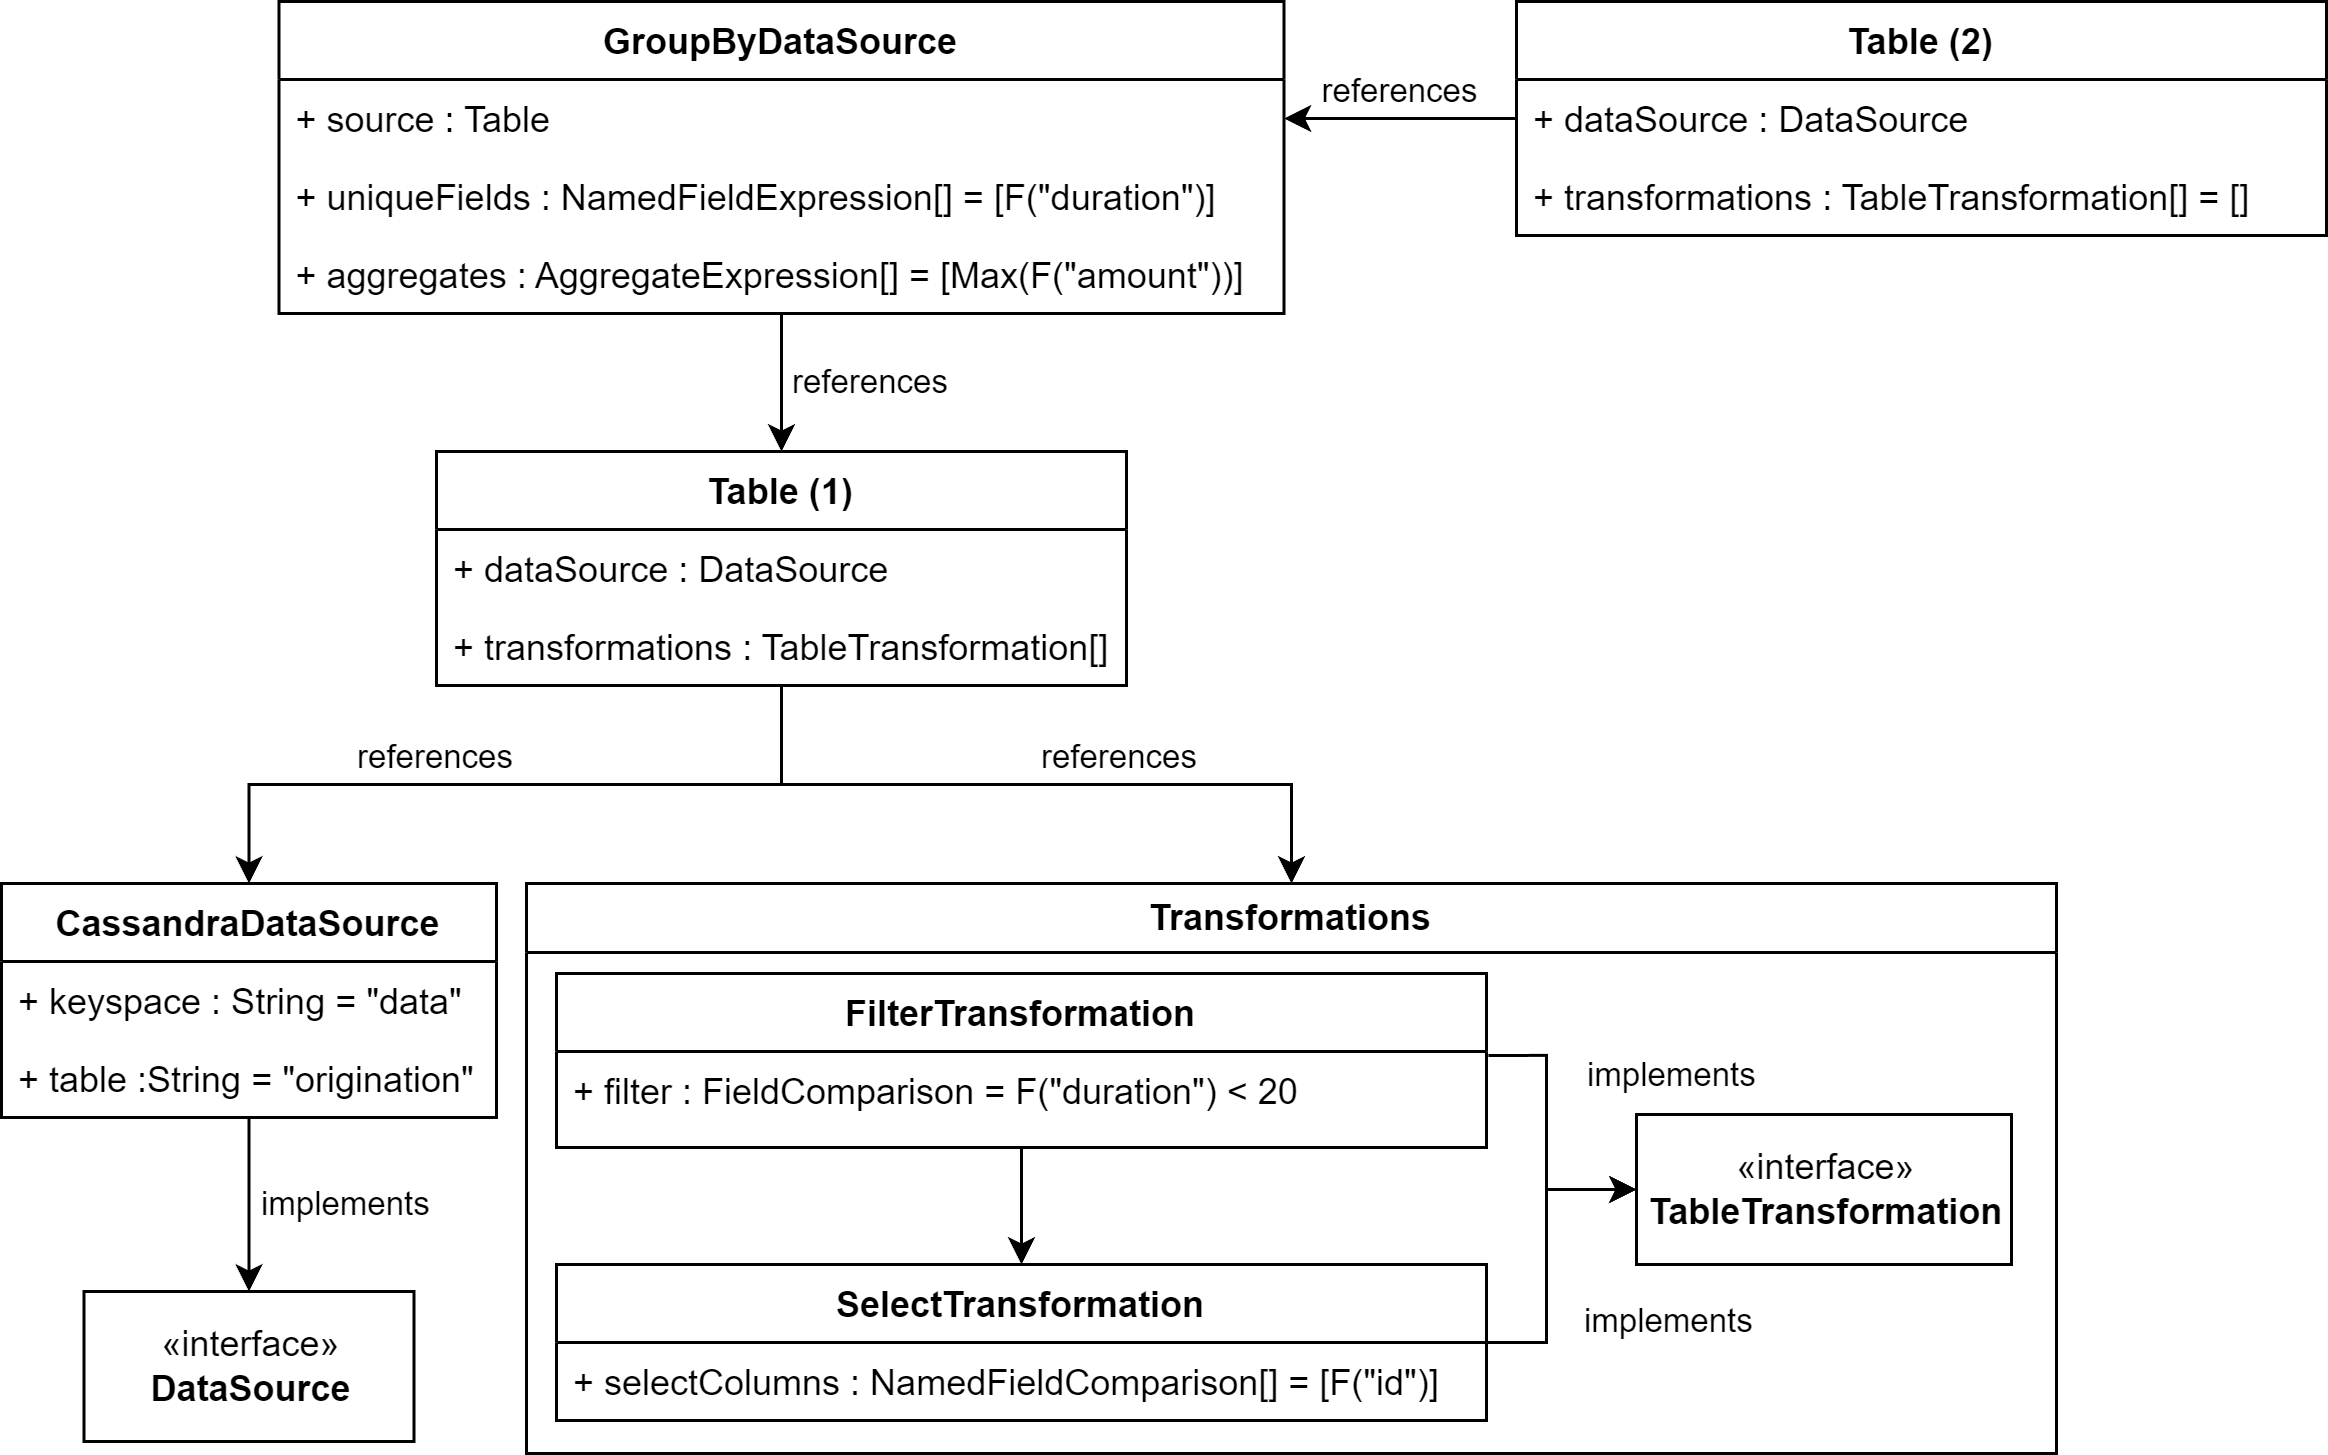
\includegraphics[width=0.8\textwidth]{chapters/diagrams/implementation/group-by-query}
	\linebreak
	\begin{python}
ClusterManager("orchestrator-service")
.cassandra_table("data", "origination")
.filter(F("duration") < 20)
.select(F("id"))
.group_by([F("duration")], [Max(F("amount"))])
.evaluate()
	\end{python}
	\caption{Example Group By Query}
	\label{fig:group-by-query}
\end{figure}

A \textit{Table} or \textit{DataSource} cannot be computed directly, but must first be split into partitions, which are provided by the \textit{DataSource}. These partitions are represented by the interface \textit{PartialDataSource}, with the partitioning method being specific to each implementation. The \textit{Table} class has a similar partial form, \textit{PartialTable}, which references a \textit{PartialDataSource} and can be computed directly. Both \textit{PartialDataSource} and \textit{PartialTable} always hold a reference to the complete version of themselves. To demonstrate how to produce a final result from a set of partial results, Figure \ref{fig:partial-filter-select-query} shows a high level example of one possible way of partitioning and computing the previous Filter and Select query.

\begin{figure}[h]
	\centering
	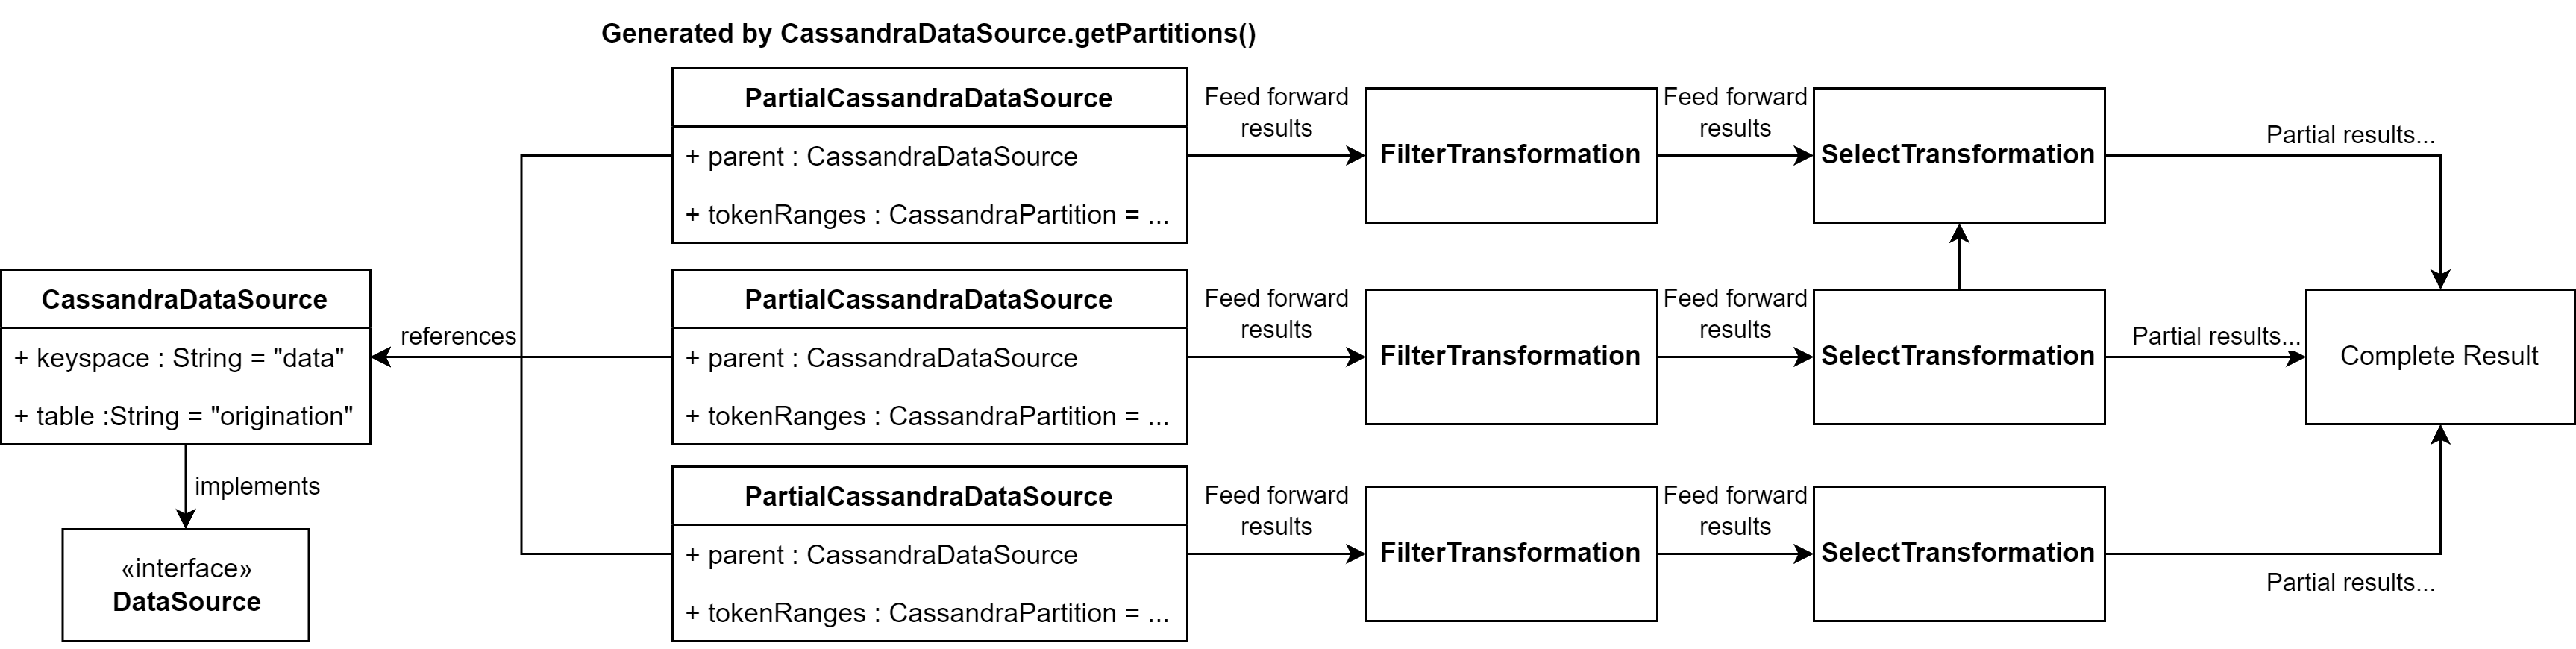
\includegraphics[width=\textwidth]{chapters/diagrams/implementation/partial-filter-select-query}
	\caption{Example Filter and Select Query}
	\label{fig:partial-filter-select-query}
\end{figure}



\section{Data Store}
The data store is the most important component for the worker implementation. It allows the workers to store partially computed data, which can be reused in later parts of the query execution. In particular when workers are communicating with one another, it is likely that the worker will be processing more than one request at the same time, which presents issues with handling concurrency and synchronisation.

The approach taken to solve this uses the actor model, first introduced in 1973 by Carl Hewitt \cite{hewitt1973session}. Specifically, the Akka Actors framework was chosen as an implementation of the actor model in Scala \cite{akkaactors}. The actor model abstracts away the complexity of synchronisation and thread management. Instead, components of the system become actors. Each actor defines a set of messages that it accepts, and the response to each message, and the framework provides a guarantee that an actor will only ever process one message at a time.

The data store is modelled as an actor which stores results as key-value pairs. Three kinds of data can be used as keys for storage: \textit{Table} computation results, \textit{DataSource} computation results and hashed data results, which are used in the process of computing a Group By partition. 

For each supported type of data, the data store uses a two-stage lookup, internally implemented using nested HashMaps. First, the full version of the data (\textit{Table} or \textit{DataSource}) is looked up, then the partial version (\textit{PartialTable} or \textit{PartialDataSource}). Partial forms of \textit{Tables} and \textit{DataSources} always contain a reference to the full version, but not the other way around. Therefore, this decision does not increase the time taken to insert new data significantly, but it is particularly useful when fetching the results for a \textit{Table}, or removing a \textit{Table} or \textit{DataSource}. Without this approach, completing these operations would require searching the entire Map to find any matches, turning the O(1) lookup time into O(n).

\subsection{Spill to Memory}
In situations with very large datasets, the amount of memory available to the workers will be less than the amount of data the system attempts to load. In this case, it is likely that the JVM will run out of heap space, causing a crash when it attempts to allocate more memory to store data. Therefore, the system features a module which allows it to move cached data onto disk to free up heap space. This module is part of the data store, and functions transparently to the rest of the system - data store queries are the same whether the result is held in-memory or on-disk.

\paragraph{Storage Interface}
To implement the spill process, an interface \textit{StoredTableResult} is defined. This interface holds a key which corresponds to that result, and a \textit{get} operation to retrieve the result data. There are two main subclasses that implement this interface: \textit{InMemoryTableResult} and \textit{ProtobufTableResult}. 

\textit{InMemoryTableResult} is a simple wrapper for the interface, which simply contains the result and holds it in memory. It also features a \textit{spillToDisk} method which moves the data onto disk by creating a file under a randomised folder name for that execution, with the name set to the hashcode of the key. 

\textit{ProtobufTableResult} only holds a pointer to the data on disk, and reads the data from there when the \textit{get} operation is called. It also features a cleanup method which removes the stored data from disk.

\paragraph{Spill Process}
The data store is responsible for managing in-memory and on-disk data. Before almost every operation on the data store, it makes a check for the current memory utilisation, which is calculated using a set of methods on the \textit{Runtime} class \cite{javaruntimeclass}. If the memory utilisation is over a given threshold, the data store attempts to spill at least the amount of bytes over the utilisation threshold. 

Figure \ref{fig:bytes-over-memory-threshold} shows how the amount of bytes over a percentage threshold is calculated. The division on the left calculates the current memory utilisation percentage, then the threshold is subtracted to get the percentage amount over it. This is multiplied by the total number of bytes to get the number of bytes that the percentage represents.

\begin{figure}[h]
	\centering
	\[ \left( \frac{\text{Bytes in Use}}{\text{Total Bytes Available}} - \text{Threshold} \right) * \text{Total Bytes Available} \]
	\caption{Number of Bytes Over Memory Threshold}
	\label{fig:bytes-over-memory-threshold}
\end{figure}

To perform the spill, the data store will follow the decision tree shown in Figure \ref{fig:spill-to-disk-process} After the process is completed, the data store forces the JVM to perform Garbage Collection to immediately free the relevant amount of memory.

\begin{figure}[h]
	\centering
	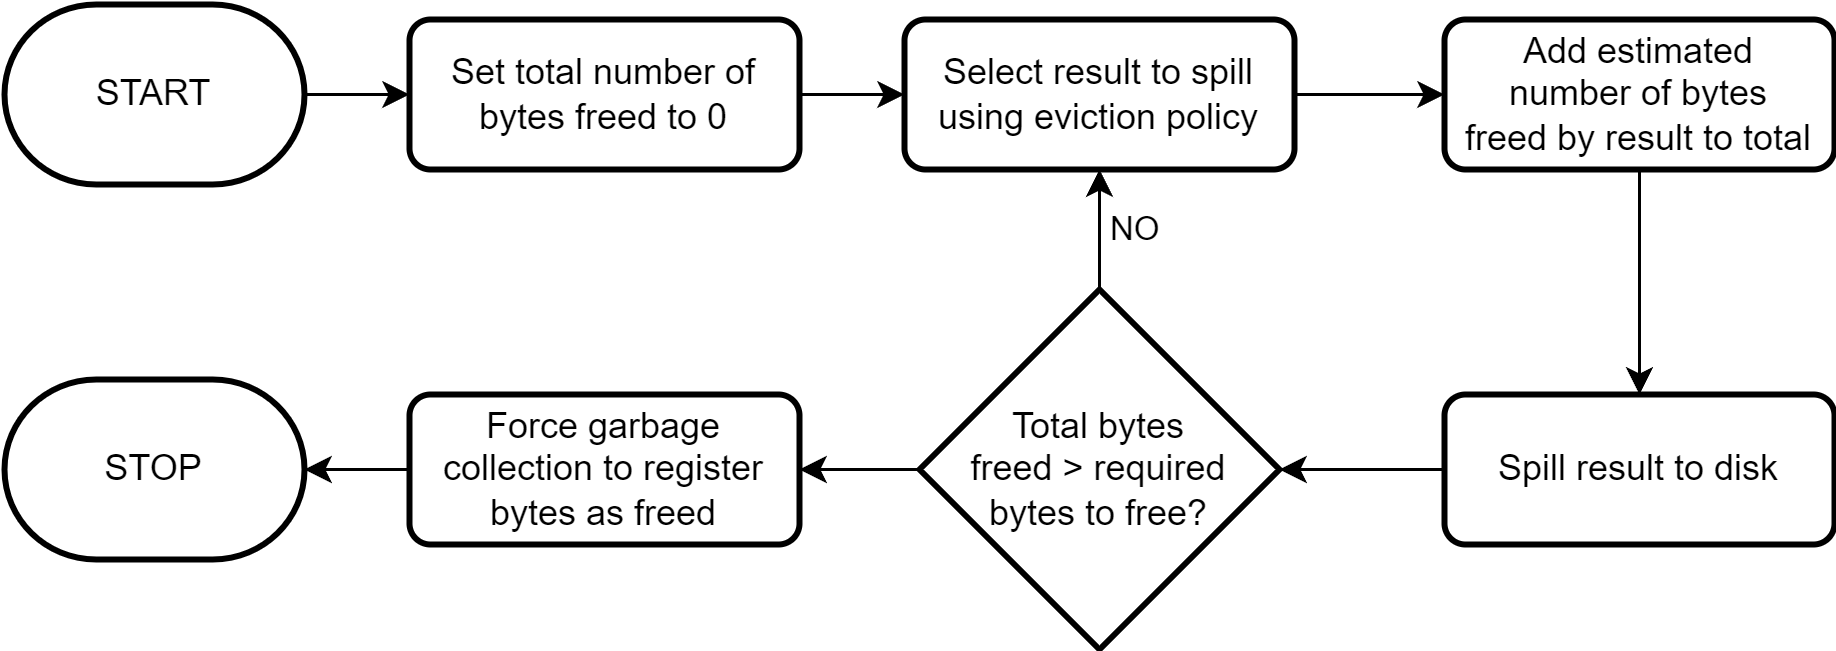
\includegraphics[width=0.6\textwidth]{chapters/diagrams/implementation/spill-to-disk-process}
	\caption{Spill to Disk Decision Tree}
	\label{fig:spill-to-disk-process}
\end{figure}

This process is not without flaws. It relies on no other class in the current JVM instance holding references to any of the results being spilled. In the controlled worker environment, it is possible to ensure this is the case, meaning the spill works reliably, but this approach would not work more generally. Also, this approach is reliant on size estimates, meaning the actual amount of memory freed will not be the same as the estimated memory freed. With a suitably low threshold for spilling (60-70\% of maximum memory) and regular checks of memory utilisation, this risk does not become a real problem.

\paragraph{Eviction Policy}
Finally, the policy for determining results to spill is important. A policy that does not fit the way the results are being used could result in large performance impacts, as it could cause antipatterns like the data store spilling a result, then immediately reading it back to memory.

The data store makes use of a least-recently-used (LRU) policy to determine the next result to spill to disk, implemented using an ordered list containing all in-memory results. When results are inserted into the data store, they are added to the end of the list. When results are read from the data store, they are moved to the end of the list. Then, when a result must be selected for spill, the item at the head of the list is chosen and removed.



\section{Partitioning}
One of the most important jobs of the orchestrator during a computation is to calculate partitions. There are two situations where partitions need to be calculated: when pulling source data from Cassandra, and when computing a Group By. The overall goal is to split the dataset into roughly equal chunks of a manageable size. 

\subsection{Cassandra}
As described in the Design Chapter, Cassandra was selected as the persistent storage module because its storage model closely matches the type of partitioning the system requires. The Cassandra \textit{DataSource} getPartitions method investigates the source data in the database, and generates an appropriate number of partitions. This process is described below.

When data is stored in Cassandra, the primary key of each row already has a 64-bit token assigned to it. Cassandra allows queries to filter on ranges of these tokens, meaning the data can be split up and read from the database in chunks. To be able to ensure the partitions are a manageable, defined size, an estimate of the size of the full source data is required. Cassandra provides this information in the \texttt{system.size\char`_estimates} table. This table provides an estimate of the size of each table in the database, and these are generated automatically every 5 minutes.

From a size estimate of the full table, estimates can be calculated for any given token range using the equation in Figure \ref{fig:token-range-estimation}. The fraction calculates the percentage of all tokens that the given token range represents.

\begin{figure}[h]
	\centering
	\[ \frac{\text{Number of Tokens in Token Range}}{\text{Total Number of Tokens: } ((2^{63}-1) - (-2^{63}))} \times \text{Estimated Table Size} \]
	\caption{Token Range Size Estimation Equation}
	\label{fig:token-range-estimation}
\end{figure}

Using this equation, it first gathers the token ranges which each node is responsible for storing. Then, it performs a joining and splitting process over each node, depending on the size of the token ranges. The set of token ranges produced after this process are the partitions used during the computation. The flowchart in Figure \ref{fig:cassandra-partitioning-decision-tree} shows the full process for generating the output partitions, 

\begin{figure}[h]
	\centering
	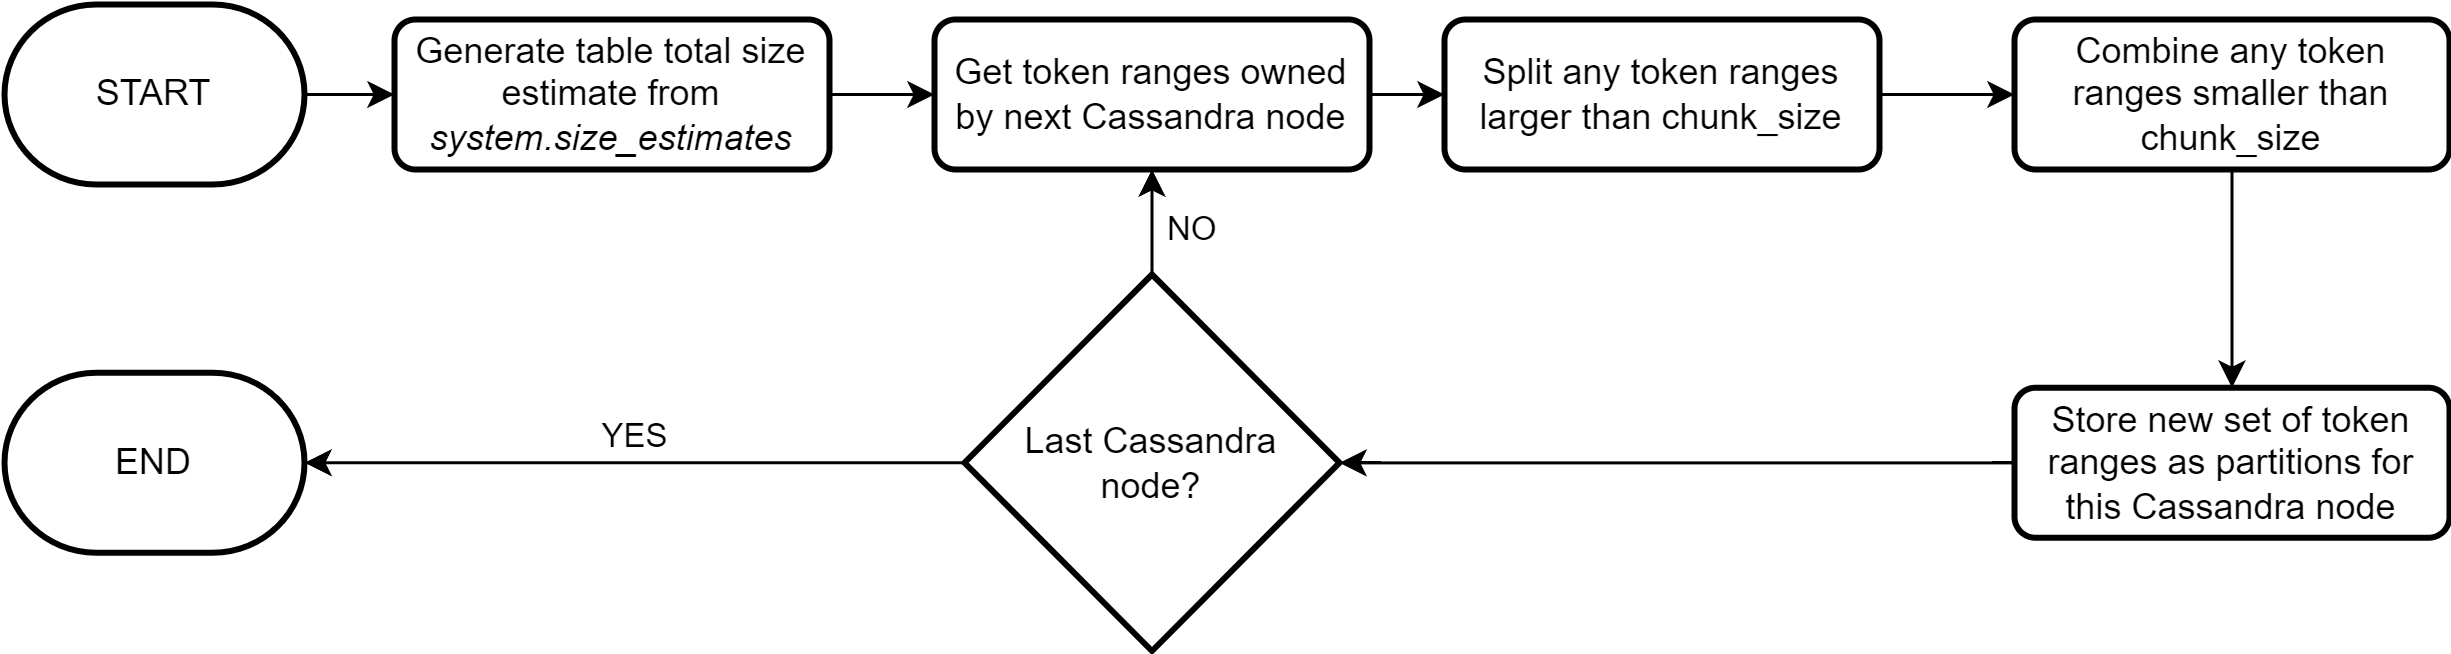
\includegraphics[width=0.8\textwidth]{chapters/diagrams/implementation/cassandra-partitioning-decision-tree}
	\caption{Cassandra Partitioning Process}
	\label{fig:cassandra-partitioning-decision-tree}
\end{figure}


Figure \ref{fig:cassandra-split-process} demonstrates how the splitting process works. The system calculates how much times larger the token range currently is than the goal partition size, then divides the token range evenly by that amount.

\begin{figure}[h]
	\centering
	\subfloat[\centering Equation]{\raisebox{1.5cm}{$ \text{Number of Splits} = \frac{\text{Token Range Size}}{\text{Chunk Size}} $}}
	\qquad
	\subfloat[\centering Example]{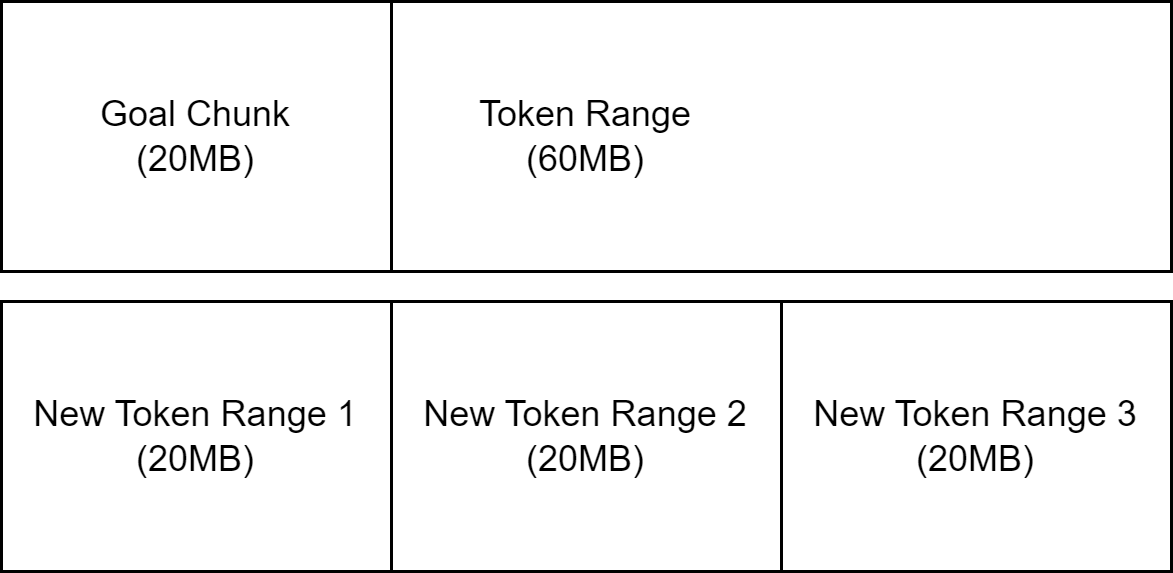
\includegraphics[width=0.4\textwidth]{chapters/diagrams/implementation/cassandra-split-example}}
	\caption{Token Range Splitting}
	\label{fig:cassandra-split-process}
\end{figure}

Figure \ref{fig:cassandra-join-process} provides an example how the joining process works. Given a sorted list of token ranges, the system repeatedly adds sequential elements to a partition until it is larger than the goal partition size. Then, the partition is marked as completed. The list is sorted by size ascending to ensure the smallest number of partitions are created - if there are a large number of very small token ranges, these will be combined into a single large partition together.

\begin{figure}[h]
	\centering
	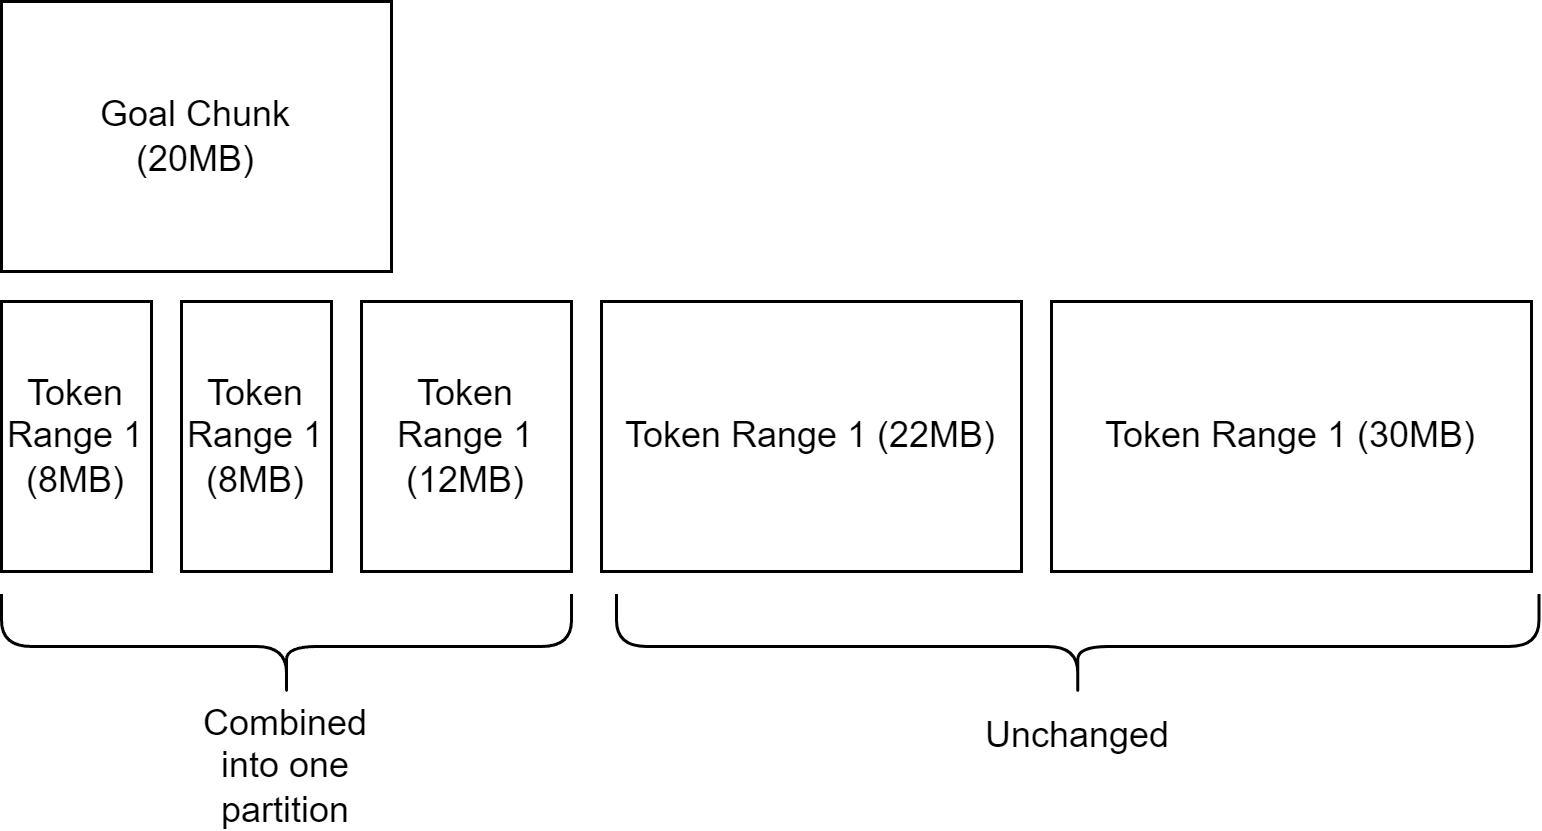
\includegraphics[width=0.5\textwidth]{chapters/diagrams/implementation/cassandra-join-example}
	\caption{Token Range Joining Example}
	\label{fig:cassandra-join-process}
\end{figure}

The Cassandra Java Driver provides a wide range of helper functions for performing the joining and splitting of token ranges accurately to produce new token ranges. The system simply calculates how much joining or splitting is required based on the size of the token ranges and the table size estimate. It then uses the driver to perform the calculations.

\subsection{Cassandra Data Co-Location}\label{subsec:colocation}
Once the list of partitions for each Cassandra node are generated, the system attempts to co-locate workers to Cassandra nodes. The goal of this process is to produce an \textit{optimal assignment} of partitions, where each partition is matched to one or more workers to minimise network latency when fetching the data from Cassandra.

To do this, each worker first calculates its closest Cassandra node. This is done by opening a TCP connection multiple times with each Cassandra node, and averaging the time taken over multiple attempts. The node with the lowest average latency is selected as the closest node. The orchestrator uses this information to match each worker to a Cassandra node and its corresponding list of partitions. The output is an optimal assignment between workers and partitions. It is possible for more than one worker to be matched to the same set of partitions, and it is also possible for a set of partitions to have no co-located worker nodes. In this case, they are kept as unassigned, and the work assignment algorithm handles their allocation. Figure \ref{fig:optimal-assignment-example} shows an example cluster setup with three physical nodes, and the optimal assignment after this process is complete.

\begin{figure}[h]
	\centering
	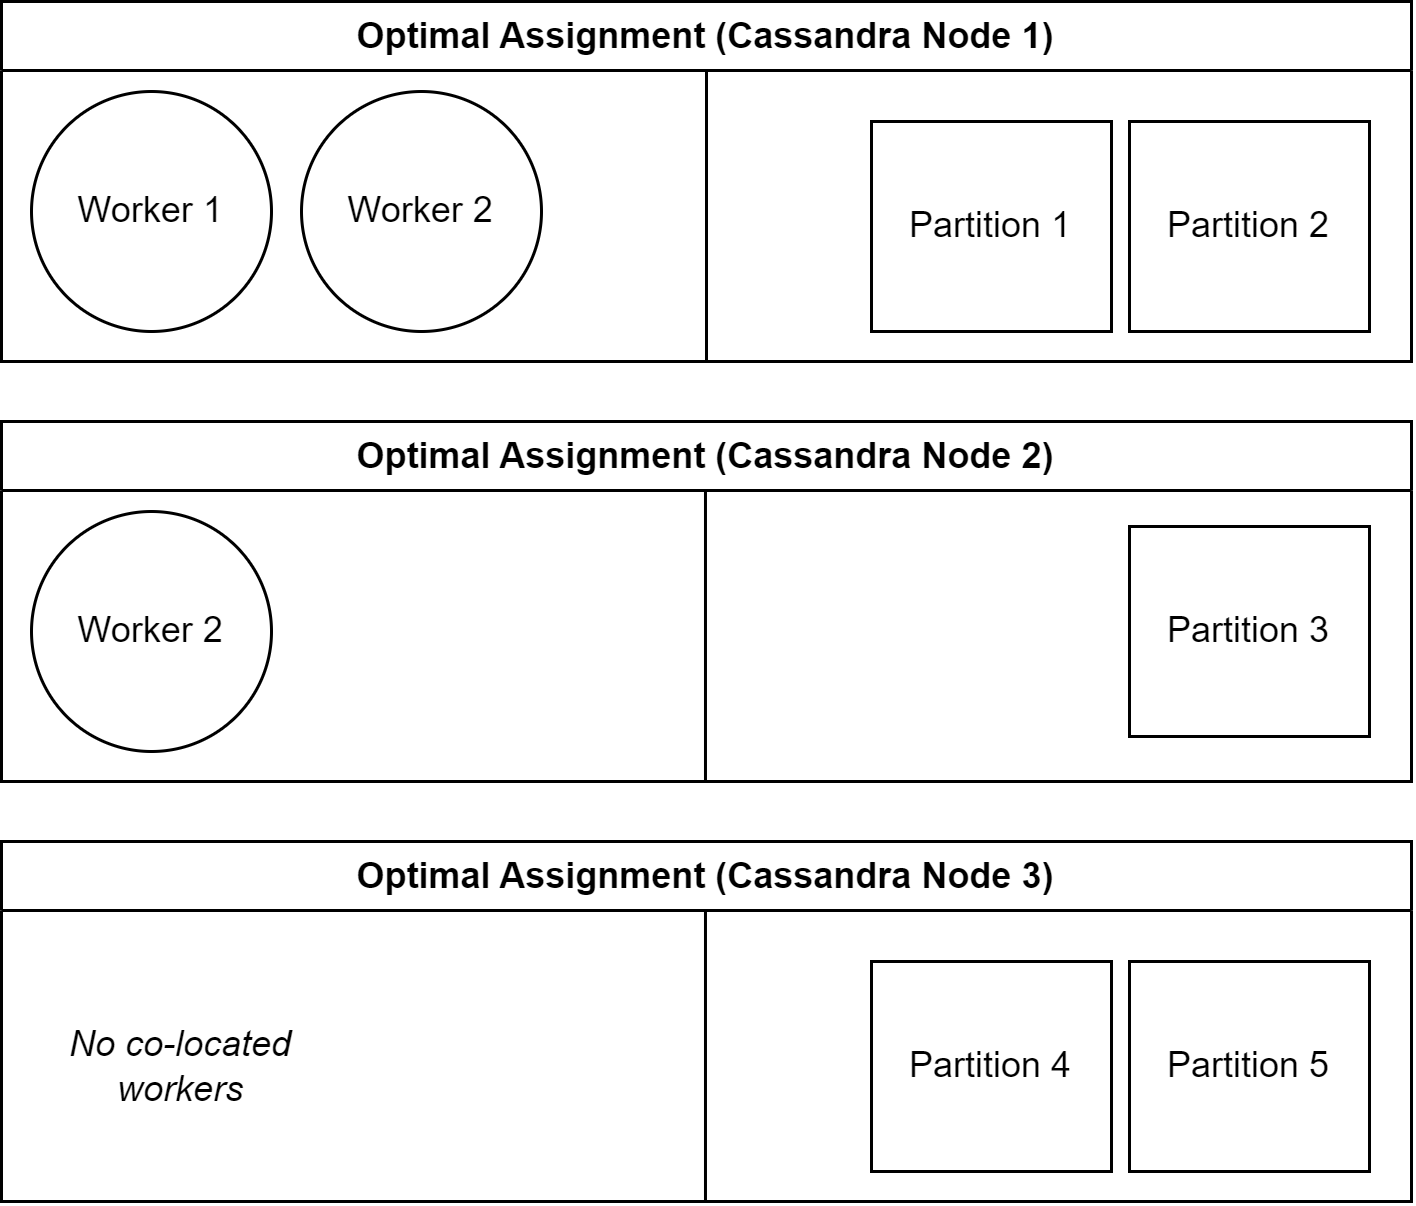
\includegraphics[width=0.8\textwidth]{chapters/diagrams/implementation/optimal-assignment-example}
	\caption{Optimal Assignment Example}
	\label{fig:optimal-assignment-example}
\end{figure}

\subsection{Group By}\label{subsec:group-by}
The Group By operation takes any number of \textit{NamedFieldExpressions} to act as unique keys, as well as any number of \textit{AggregateExpressions} which will be computed for each combination of unique keys. As with pulling source data from Cassandra, the goal when computing a Group By is for the partitions generated to be roughly equal chunks of a manageable size. To do this, two things are needed: an estimate of the full size of the dataset, and a way of splitting the dataset up to keep unique keys together. 

The process of calculating partitions and hashes, shuffling data, computing the result and deleting the original hashes is all controlled by the orchestrator during Query Plan Execution.

\paragraph{Partitions}
The first step is to compute the number of partitions that the Group By will be made up of, which is based on the size of the full dataset. To estimate this, an existing class, \textit{SizeEstimator}, was reused from Apache Spark, with some changes for compatibility with Scala 3 \cite{zaharia2016spark}. This class provides a static method \textit{estimate} which accepts any Scala object and produces an estimate, in bytes, of the size of the object. This can be called on all partial results across all workers, and the results totalled to calculate the total size of all data for a Table. Figure \ref{fig:group-by-num-partitions} shows how the size estimate can be used to derive the total number of partitions to generate for a Table.

\begin{figure}[h]
	\centering
	\[ \frac{\text{Table Size Estimate}}{\text{Goal Partition Size}} \]
	\caption{Group By - Total Partitions}
	\label{fig:group-by-num-partitions}
\end{figure}



\paragraph{Hashing} 
A unique partition is then defined as the tuple of the total number of partitions, and the partition number of this partition. Hashing, combined with the modulo operation, is used to determine which partition each row should be assigned to. In particular, Murmur3Hash is used as the hashing algorithm, which is used in Cassandra and is provided natively by Scala \cite{murmur3hash}. Figure \ref{fig:group-by-partition-assign} shows the high level equation for assigning rows to partitions. This process ensures that the new partitions will be roughly equal in size, and all rows with the same values for the unique keys will be mapped to the same partition.

\begin{figure}[h]
	\centering
	\[ Murmur3Hash(\text{Unique Key Data}) \; \%  \; \text{Total Partitions} \]
	\caption{Group By - Row Partition Assignment}
	\label{fig:group-by-partition-assign}
\end{figure} 

\paragraph{Computation}
After the hashes are computed and a worker is assigned a particular partition, it must communicate with all other workers in the cluster to get any data that relates to that partition.This ensures that the partition data is complete, and it is much the same as when the orchestrator requests query result data from the workers. The worker makes a request to all other workers, and they stream the header and rows of their partial data back to the worker that made the request. When a Group By is being computed, it's likely that a worker will be simultaneously receiving data from another worker, and sending a different set of data to it. This makes the actor system driving the data store in each worker particularly valuable, as it provides thread-safe concurrent access to the data store.

Once a worker has collected all data relating to a particular partition, it must compute the Group By result. Scala features a built-in Group By function, which this operation uses. The values for the unique keys of the Group By are calculated for each row, and the rows are placed into groups based on those values. Then, the aggregate functions are computed for each of the groups, resulting in one output row for each combination of unique keys. 

\paragraph{Deletion}
Finally, the last step of computing a Group By is to remove the hashed partition data stored on each worker, as it is no longer needed. This is handled by the orchestrator automatically during the process of computing the Group By \textit{DataSource.}

\section{Row-Level Computations}
Once partitions have been delegated to the workers, performing the computation is relatively straightforward. Included below are descriptions of how the Select and Filter operations are performed.

\subsection{Select} 
This operation takes any number of \textit{NamedFieldExpressions}. To compute a result, each \textit{NamedFieldExpression} is applied to each row of the input result. The output result has the same number of rows as the input, and fields equal to the number of \textit{NamedFieldExpressions}. 

\subsection{Filter}
This operation takes a single \textit{FieldComparison}, or a number of \textit{FieldComparisons} combined using boolean operators. To compute, each comparison is applied to each row of the input result, removing any rows where the comparison returns \texttt{false}.



\section{Query Plan}
Query plans are the process through which the orchestrator can calculate how to get from a query written by the user, to a result which it can return. A Query Plan is made up of a sequence of \textit{QueryPlanItems}, which is an interface defining one part of a query plan. Each \textit{QueryPlanItem} has an \textit{execute} method, which will make some change to the state of all workers in the cluster when called. There are four main QueryPlanItem implementations, which allow \textit{DataSources} and \textit{Tables} to be calculated and deleted.

Both \textit{DataSource} and \textit{Table} have a function that generates the full Query Plan to compute their output from scratch, as well as a second Query Plan to clean any result in the data store. 

Figure \ref{fig:filter-group-by-query-plan} shows the query plans for the Filter and Select query (\ref{fig:filter-select-query}) and Group By Query (\ref{fig:group-by-query}).

\begin{figure}
	\centering
	\subfloat[\centering Filter and Select Query]{{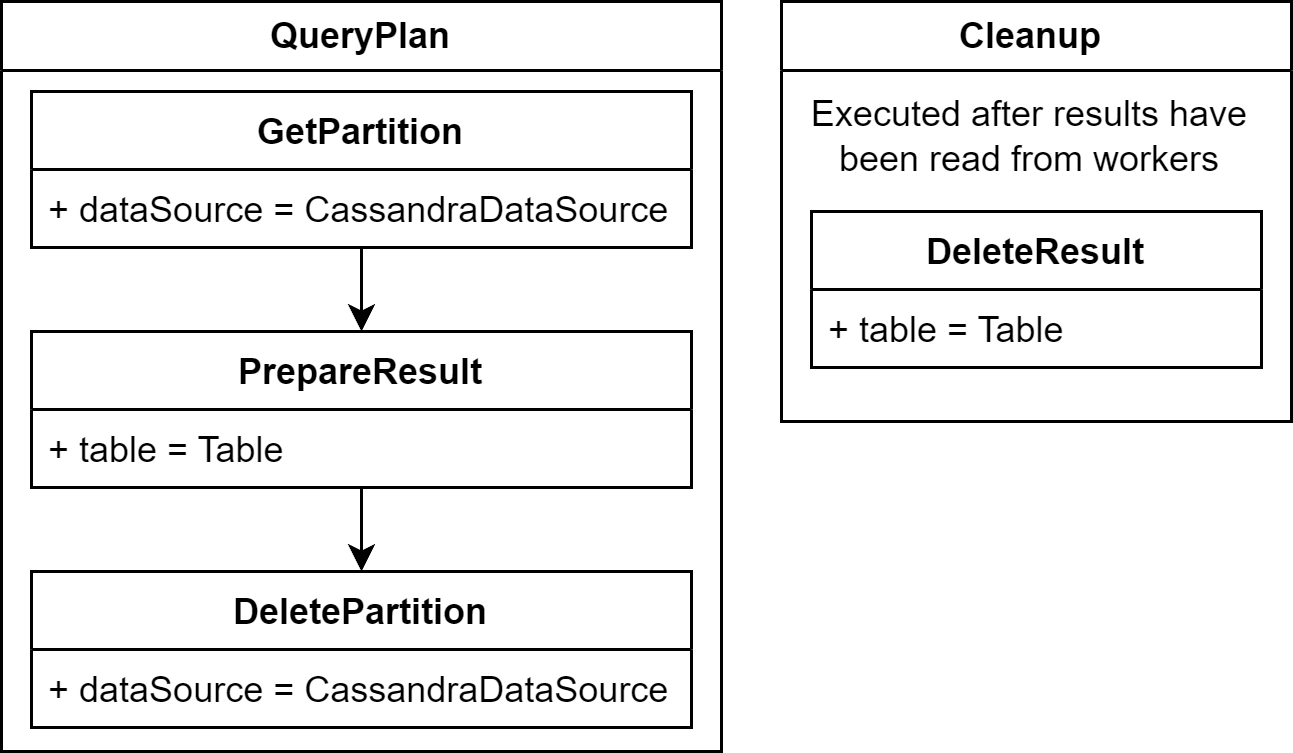
\includegraphics[width=0.3\textwidth]{chapters/diagrams/implementation/filter-select-query-plan}}}
	\qquad
	\subfloat[\centering Group By Query]{{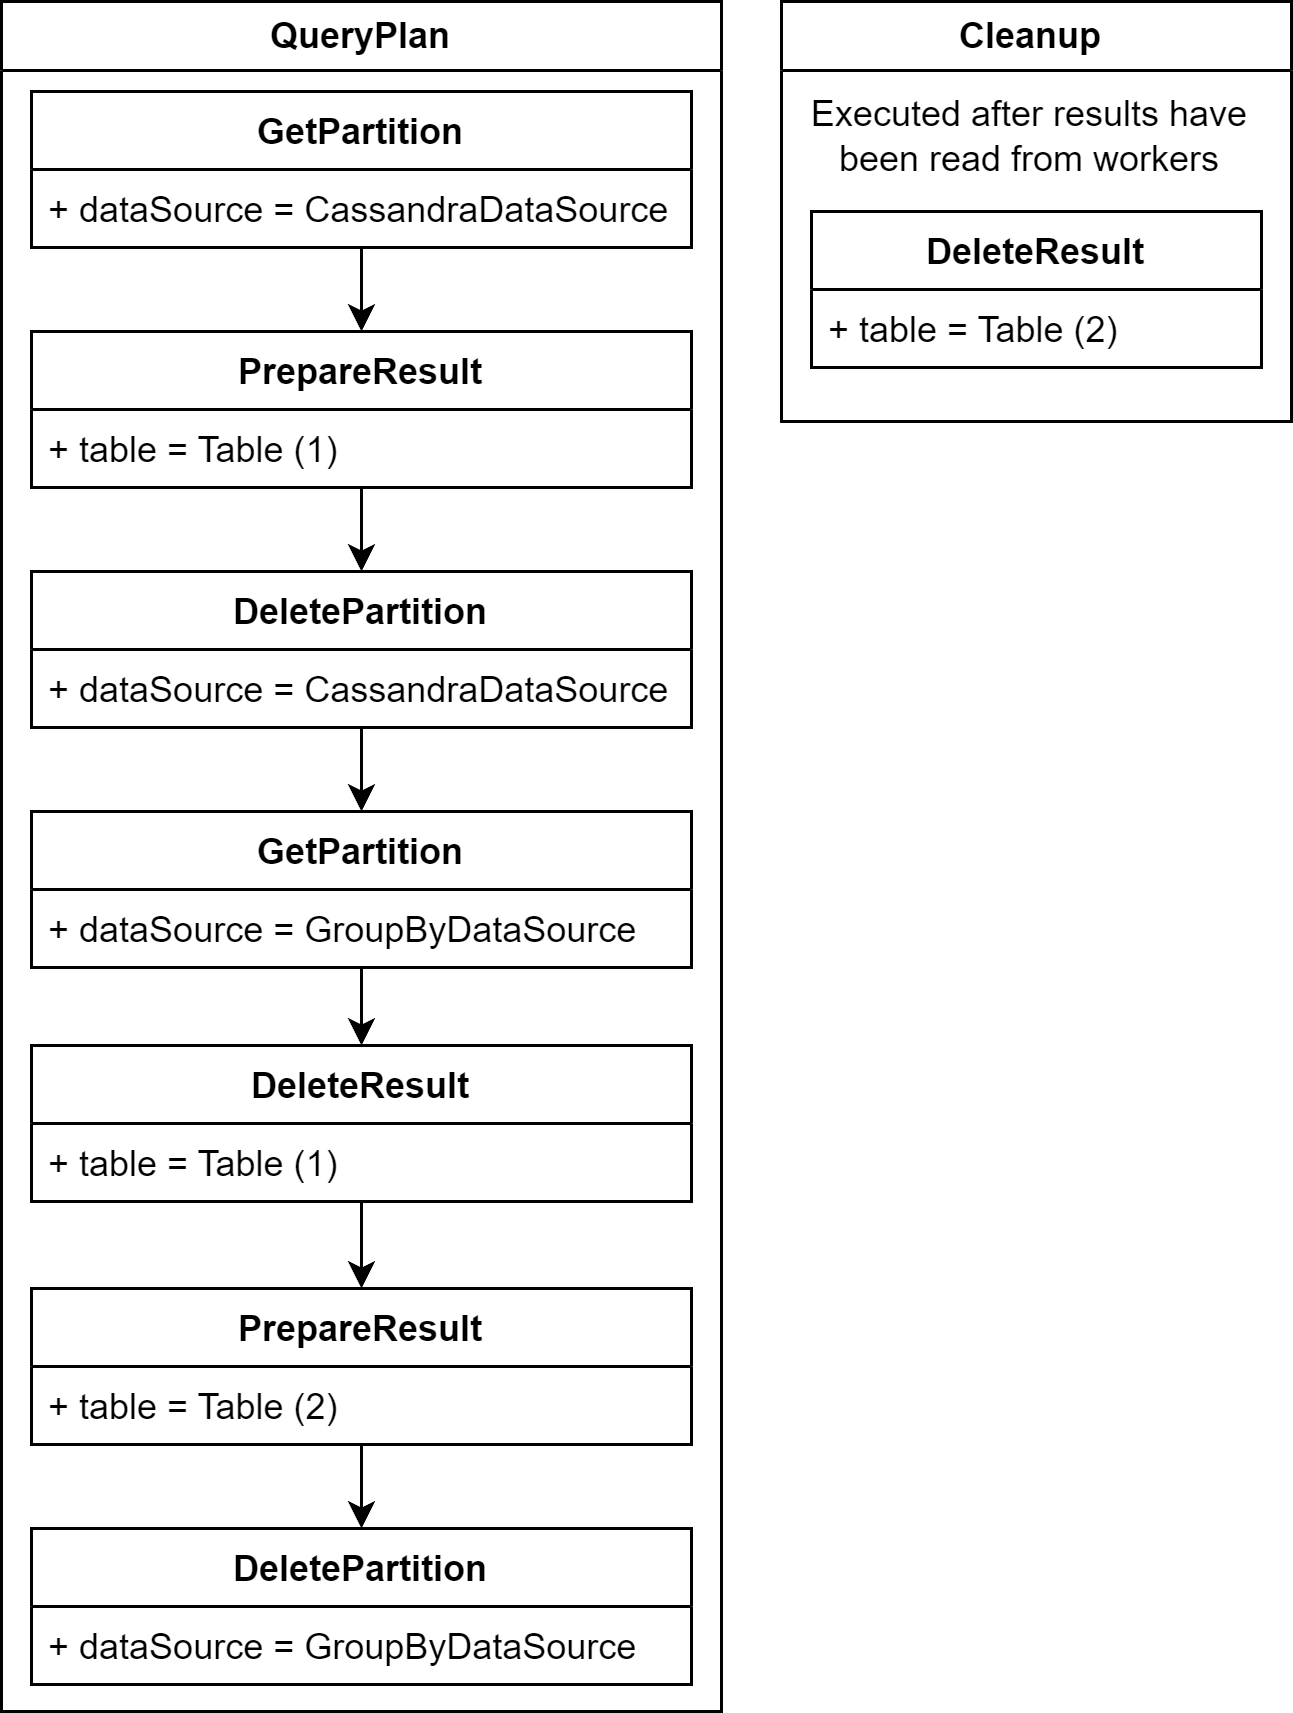
\includegraphics[width=0.3\textwidth]{chapters/diagrams/implementation/group-by-query-plan}}}
	\caption{Query Plans - Filter-Select and Group By Query}%
	\label{fig:filter-group-by-query-plan}
\end{figure}

\subsection{GetPartition}
This is the most complex \textit{QueryPlanItem}, encapsulating a number of steps in order to compute and store the partitions of a \textit{DataSource}. There are two main flows depending on if the \textit{DataSource} has dependent Tables.

If the \textit{DataSource} has no dependencies, for example when pulling data from Cassandra, then Figure \ref{fig:get-partition-no-dependencies} shows the process for this item. 

\begin{figure}[h]
	\centering
	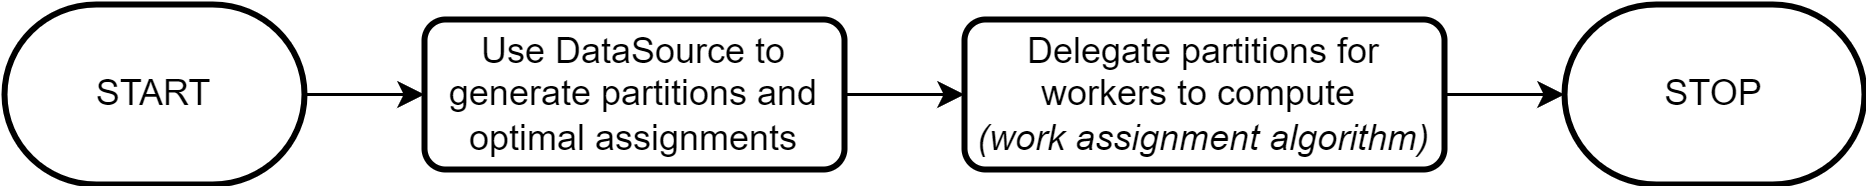
\includegraphics[width=0.8\textwidth]{chapters/diagrams/implementation/get-partition-no-dependencies-flow}
	\caption{Get Partition Execution - Without Dependencies}
	\label{fig:get-partition-no-dependencies}
\end{figure}

If the \textit{DataSource} has dependencies, then Figure \ref{fig:get-partition-dependencies} shows the process for this item. First, the partitions and optimal assignments are generated, then the dependency data is hashed based on the number of partitions to generate. Both of these steps are implementation-specific, and are therefore abstracted behind the \textit{DataSource} interface. The work assignment algorithm is then run to delegate partitions to the workers, followed by deleting the hashed dependency data. These steps do not change based on the \textit{DataSource}, so are handled exclusively by \textit{GetPartition}. These steps are the same as when calculating a Group By (Section \ref{subsec:group-by}), which is an implementation of \textit{DataSource}.

\begin{figure}[h]
	\centering
	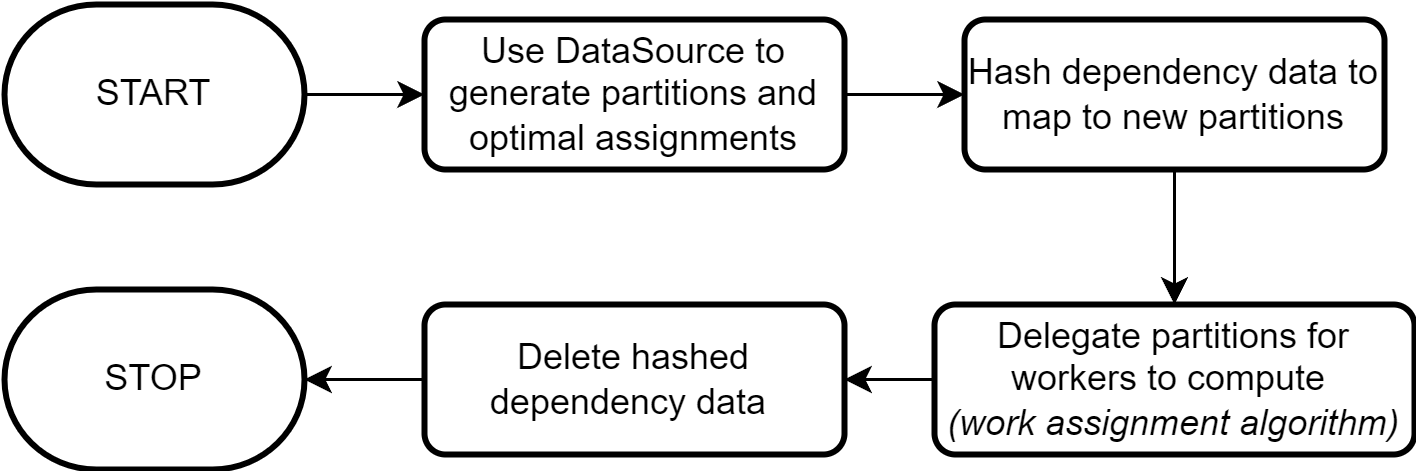
\includegraphics[width=0.7\textwidth]{chapters/diagrams/implementation/get-partition-dependencies-flow}
	\caption{Get Partition Execution - With Dependencies}
	\label{fig:get-partition-dependencies}
\end{figure}

\paragraph{Work Assignment Algorithm}
The details of how the partitions are actually computed are abstracted behind the \textit{DataSource} interface as they are implementation specific, but GetPartition always needs to manage the process of sending requests to the workers to compute the partitions. This is done using the Work Assignment Algorithm. 

A simple solution would be to use a round-robin process to match optimal assignments to their workers, delegating work when a request finishes and stopping when the assignment list is empty. However, this can result in idle workers, for example if one worker's list of optimal assignments is shorter than the others, or if one worker takes unexpectedly long to complete their work.

The ideal solution would ensure a worker computes all of its own optimal partitions first and, once these are complete, computes the partitions that were originally assigned to other workers. This implements a form of dynamic load balancing, because a faster-running worker is able to take on more requests than a slower worker, and no worker will be idle unless there are no partitions left to compute. However, this presents concurrency challenges, including preventing race conditions like the same partition being delegated twice to different workers.

The actor model, used previously in the data store, is ideal for this situation. Sets of optimal partitions are modelled as \textit{producer} actors, and the workers as \textit{consumers}. Producers respond to requests for work with partitions to be computed. Consumers are provided with an ordered list of producers, then repeatedly request and compute work from each in order. Each consumer is given a differently ordered list, with the producer of that consumer's optimal partitions placed first in the list. When all assigned producers for a consumer are empty, the consumer will shut down. The final part of the system is a counter, which tracks the number of completed partitions, sending a signal when all partitions have been computed, or an error if any worker fails.

This solution also handles the case where no worker is co-located with a set of partitions; this producer will simply be placed last in the list of producers for each consumer, resulting in these partitions eventually being processed.

Figure \ref{fig:producer-consumer-model-example} provides the initial state of this model, using the example optimal assignment in Figure \ref{fig:optimal-assignment-example}. Dark arrows represent the producer which the consumer will empty first, containing its optimal assignments. Light grey arrows represent the other producers which the consumer can access. Note that Producer 3 is not the first producer for any worker, but will eventually be checked by the workers when all other producers are exhausted.

\begin{figure}[h]
	\centering
	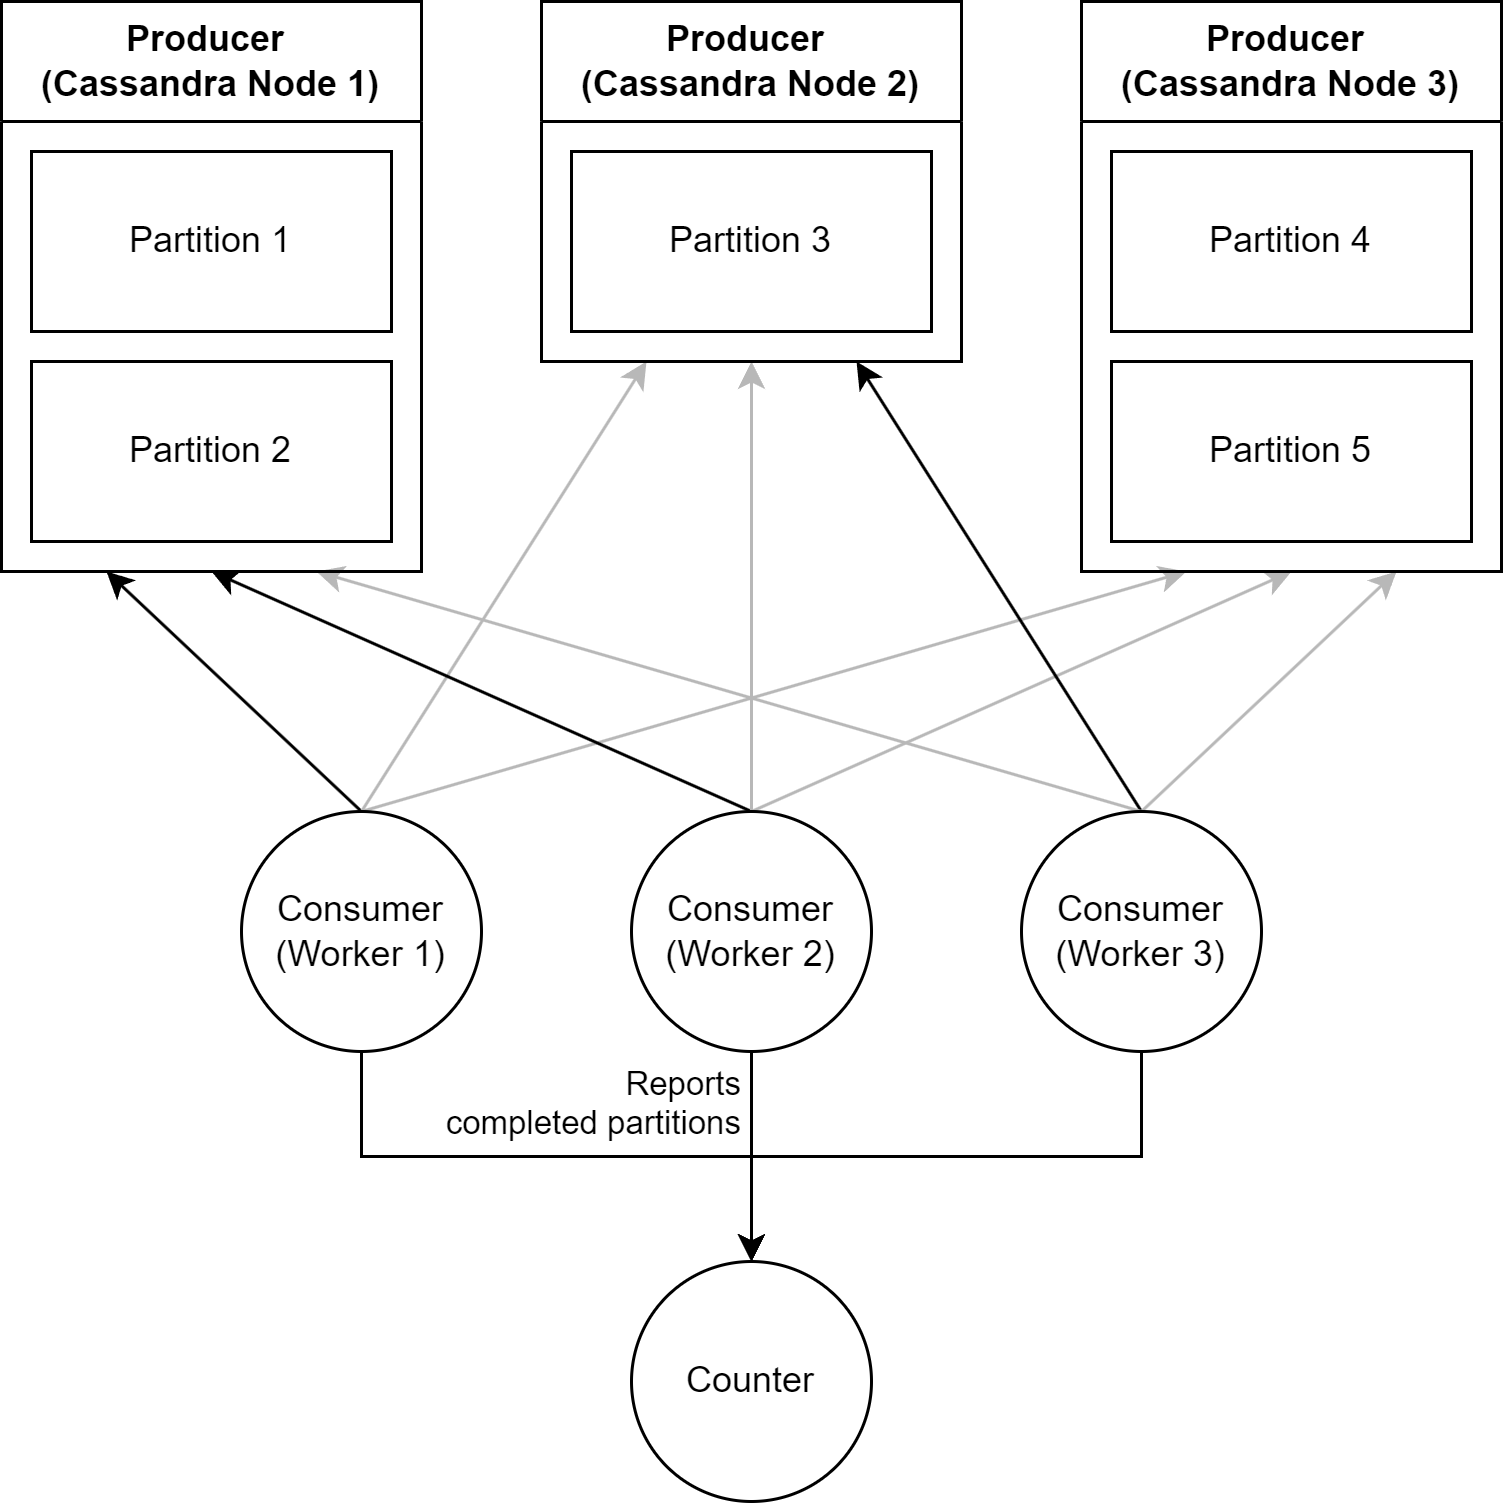
\includegraphics[width=0.5\textwidth]{chapters/diagrams/implementation/producer-consumer-model-example}
	\caption{Producer Consumer Model Example}
	\label{fig:producer-consumer-model-example}
\end{figure}

\subsection{PrepareResult}
This \textit{QueryPlanItem} computes a Table from the partitions of a \textit{DataSource} that are already stored on the workers. Therefore, it will always be called after GetPartition, with the partitions generated by \textit{GetPartition} as an argument. The implementation uses a modified version of \textit{GetPartition}'s actor system, which iterates through all partitions on each worker, sending a request for each partition to perform the \textit{Table} computation.

\subsection{DeleteResult and DeletePartition}

\textit{DeletePartition} and \textit{DeleteResult} are \textit{QueryPlanItems} for removing the results of a \textit{GetPartition} and \textit{PrepareResult} operation, respectively. These will send a single request to each worker, and they will remove all results that relate to a \textit{Table} or \textit{DataSource}, and respond with a confirmation.

\subsection{Result Collation}
After all the steps of a query are completed, the final results are stored across all the workers. The orchestrator makes a request to all workers to return the computed results, and each worker iterates over all partial results in the data store, streaming the data back to the orchestrator. An actor system is used to pipe the concurrent responses from all workers into a single thread, which combines the results and streams them to the frontend. 

The request is initiated by the orchestrator, rather than the workers pushing data to the orchestrator, because gRPC requires that one system act as a server, and another as a client. For the query plan model, it makes most sense for the workers to be servers, so this much also be the case for result collation.

\section{Deployment}
As discussed in Chapter \ref{cha:design}, Kubernetes was chosen to manage all nodes in the cluster. One of the key features that makes it useful for the system are scheduling rules, which provide Kubernetes with information about how containers should be assigned to physical nodes.

As previously described in \ref{subsec:colocation}, worker nodes will determine their closest Cassandra node automatically based on latency. To make the best use of the cluster, workers should be distributed evenly across all nodes that have a Cassandra node, and the following two scheduling rules will provide this:
\begin{enumerate}
	\item Workers should be placed on the same Kubernetes node as a Cassandra node if possible.
	\item Workers should not be placed on the same node as other worker nodes.
\end{enumerate}

The scheduling rules are expressed as preferences rather than requirements, Kubernetes is still able to schedule the nodes if there are more workers than Cassandra nodes.

\subsection{CI/CD}
To aid in deploying to Kubernetes, continuous integration/continuous deployment (CI/CD) pipelines are used for each of the components of the system, specifically using GitHub Actions \cite{githubactions}. Each pipeline runs all unit tests for the component, and provided they succeed, builds a docker container and pushes it to a container registry, ready for use in the Kubernetes cluster.

